\documentclass[11pt]{amsart}

% Encoding and fonts
\usepackage[T1]{fontenc}
\usepackage[utf8]{inputenc}
\usepackage{lmodern}

% Math packages
\usepackage{amsmath}
\usepackage{amssymb}
\usepackage{amsfonts}
\usepackage{amsthm}
\usepackage{mathtools}

% Figures, tables, layout, and utilities
\usepackage{graphicx}
\usepackage{float}
\usepackage{booktabs}
\usepackage{array}
\usepackage{geometry}
\usepackage{enumitem}

\geometry{margin=1in}

\numberwithin{equation}{section}
\setcounter{tocdepth}{3}
\setcounter{secnumdepth}{3}

% ---------------------------------------------------------
% Theorem-like environments
% ---------------------------------------------------------
\theoremstyle{plain}
\newtheorem{theorem}{Theorem}[section]
\newtheorem{proposition}[theorem]{Proposition}
\newtheorem{lemma}[theorem]{Lemma}
\newtheorem{corollary}[theorem]{Corollary}
\newtheorem{conjecture}[theorem]{Conjecture}

\theoremstyle{definition}
\newtheorem{definition}[theorem]{Definition}
\newtheorem{experiment}[theorem]{Experiment}
\newtheorem{heuristic}[theorem]{Heuristic}
\newtheorem{question}[theorem]{Question}

\theoremstyle{remark}
\newtheorem{remark}[theorem]{Remark}
\newtheorem{warning}[theorem]{Warning}

% ---------------------------------------------------------
% Commands
% ---------------------------------------------------------
\newcommand{\RVM}{\mathrm{RVM}}
\newcommand{\diff}{\mathrm{diff}}
\newcommand{\GUE}{\mathrm{GUE}}
\newcommand{\KS}{\mathrm{KS}}
\newcommand{\rms}{\mathrm{rms}}
\newcommand{\mean}{\mathrm{mean}}
\newcommand{\median}{\mathrm{median}}
\newcommand{\Poisson}{\mathrm{Poisson}}
\newcommand{\Rayleigh}{\mathrm{Rayleigh}}
\newcommand{\Wigner}{\mathrm{Wigner}}

\title{Logarithmic Proper-Time Interference in Zeta-like Quantum Chaotic Spectra}

\author{V. Casa\~na-Giner}
\address{Universidad Nacional de Educaci\'on a Distancia, Faculty of Mathematics, Spain}
\email{vcasana1@alumno.uned.es}
\date{}

\keywords{Riemann zeta function, quantum chaos, GUE statistics, spectral interference, logarithmic proper time, Riemann--von Mangoldt formula, Rayleigh law, block coherence}

% Hyperref must be loaded last
\usepackage[hidelinks]{hyperref}

\begin{document}

\begin{abstract}
We introduce a logarithmic proper-time observable for zeta-like quantum chaotic spectra. Writing a nontrivial zero as \(\rho_k=\sigma_k+i\gamma_k\), the finite numerical transform uses the critical-line amplitude \(\sigma=1/2\), and assigns to the ordinate \(\gamma_k\) the level-dependent clock \(\tau_k=\pi\log\log k/\log k\). The resulting ordered amplitude \(S_N^\zeta=\sum_{k=3}^{N}\exp(\tau_k/2+i\gamma_k\tau_k)\) is not a spacing statistic but a phase-interference observable. The Riemann--von Mangoldt/Lambert sequence is used as a smooth semiclassical background. The one-step residual vector gaps are Rayleigh-like rather than GUE-like, with \(KS_{\rm Rayleigh}=0.083901339184571433\), \(KS_{\rm GUE}=0.27524262614727296\), and near-zero CDF exponent \(\alpha=1.9625998029380822\). The coherent signal appears only after preserving the order in \(k\) and summing consecutive windows, where the residual window excess reaches \(8.47496580076509\), \(11.848018307196\), and \(15.8890898166697\) for \(W=500,1000,2000\). A complementary counting-coordinate balance records how a supplied off-critical zero with \(\sigma_k\neq1/2\) generates a signed displacement. The article therefore separates local planar fluctuation, ordered block coherence, and real-coordinate off-critical detection.
\end{abstract}

\maketitle
\tableofcontents
\bigskip

\begin{remark}
\label{rem:mathematical_status}
This article is a mathematical-physics investigation of a finite numerical observable built from tabulated zeta-zero ordinates.  The definitions and algebraic identities below are exact for the finite data used.  Numerical statements are recorded as finite computational observations.  The physical interpretation in terms of proper time, semiclassical background, spectral response, redshift, and block coherence is heuristic unless explicitly stated otherwise.
\end{remark}

\section{Introduction}
\label{sec:introduction}

One of the major advances in the modern understanding of the Riemann zeta function came from an unexpected connection between the physics of chaotic quantum systems and the mathematics of zeta zeros.  Montgomery's pair-correlation work showed, under the Riemann Hypothesis and for a restricted test-function range, a two-point correlation law for the zeta-zero ordinates \cite{Montgomery1973}.  Freeman Dyson observed that the same limiting form occurs in the Gaussian Unitary Ensemble of random matrix theory, the ensemble that appears in quantum systems without time-reversal symmetry.  Subsequent large-scale computations by Odlyzko gave strong numerical evidence for this Montgomery--Odlyzko/GUE picture \cite{Odlyzko1987}.  This connection is now part of the standard interface between zeta zeros, random matrices, and quantum chaos; see also \cite{Berry1986,BohigasGiannoniSchmit1984,KatzSarnak1999,RudnickSarnak1996,KeatingSnaith2000,ConreySnaith2008}.

This physical background explains why a paper about zeta zeros may legitimately introduce spectral language.  The usual random-matrix description tests the sequence through unfolded spacings, pair correlations, number variance, and related observables.  These statistics examine the distribution of levels.  They do not directly test how the ordered spectrum interferes after a nonlinear phase projection.

We write a nontrivial zero as
\begin{equation}
\rho_k
=
\sigma_k+i\gamma_k,
\label{eq:introduction_zero_definition}
\end{equation}
where the ordinates are ordered increasingly.  Under the Riemann Hypothesis one has
\begin{equation}
\sigma_k
=
\frac{1}{2}
\label{eq:introduction_rh_sigma_value}
\end{equation}
for every nontrivial zero.  The computations in this article use tabulated critical-line ordinates and therefore evaluate the logarithmic proper-time transform at the critical-line amplitude parameter
\begin{equation}
\sigma
=
\frac{1}{2}.
\label{eq:introduction_computational_sigma}
\end{equation}
We then use the spectral notation
\begin{equation}
E_k=\gamma_k.
\label{eq:introduction_energy_identification}
\end{equation}
The observable studied here assigns to the \(k\)-th level a logarithmic proper time
\begin{equation}
\tau_k
=
\pi\frac{\log\log k}{\log k},
\qquad k\geq 3,
\label{eq:introduction_proper_time}
\end{equation}
and forms the complex term
\begin{equation}
z_k^\zeta
=
\exp\left(\frac{\tau_k}{2}+iE_k\tau_k\right).
\label{eq:introduction_transformed_term}
\end{equation}
The primary object is the ordered cumulative amplitude
\begin{equation}
S_N^\zeta
=
\sum_{k=3}^{N}z_k^\zeta.
\label{eq:introduction_primary_sum}
\end{equation}
The word ordered is essential.  The observable is not the unordered cloud of the points \(z_k^\zeta\).  It is the cumulative interference produced by the spectral sequence in its natural order.

The smooth comparison sequence is obtained from the Riemann--von Mangoldt/Lambert approximation.  We denote the corresponding background ordinates by
\begin{equation}
E_k^{(0)}=\gamma_k^{\RVM}.
\label{eq:introduction_rvm_background}
\end{equation}
The RVM/Lambert sequence is used as a semiclassical background: it supplies the smooth Weyl-type spectral skeleton against which the true zeta fluctuation is measured.

The main finite observation is that the individual transformed zeta and RVM terms may be close at the term-cloud scale, whereas their ordered cumulative sums are sharply different.  The residual sequence is locally simple but globally ordered: its one-step vector gaps are Rayleigh-like, while its ordered window sums exhibit large coherent excess.


From the mathematical side, the point of the construction is that it is an exponential sum over zeta-zero ordinates which reveals a complex ordered morphology and a strong separation between the smooth RVM background and the true zeta response.  Standard exponential sums over zeros, explicit-formula sums, fractional-part statistics, and random-matrix spacing observables form a large literature.  However, within the literature cited here, and to the author's knowledge, no published exponential-sum observable has isolated a comparable finite morphology in which the RVM/Lambert control is small and smooth while the zeta transform develops a two-nucleus, arm, and tube structure under the same deterministic weight.  This is therefore presented as a new class of zeta observables: ordered phase-interference observables governed by a visible but not yet analytically characterized law of block coherence.

This viewpoint is not limited to zeta zeros.  Any system with an ordered quantum chaotic spectrum, a smooth semiclassical background, and a physically meaningful level-dependent clock can be tested by the same construction.  The article is therefore also a model for underexplored spectral approaches in which one studies not only level statistics, but ordered proper-time interference.

\begin{remark}
\label{rem:introduction_physics_link}
The physical systems motivating the language are described in Section \ref{sec:physical_systems}.  The relevant examples are quantum chaotic spectra, random-matrix spectra, trace-like spectral amplitudes, and effective scale geometries.  The role of zeta in this article is spectral: the zero ordinates are used as a model quantum chaotic spectrum.
\end{remark}

\section{Standard background and status of the present observable}
\label{sec:standard_background_status}

\begin{remark}
\label{rem:standard_material}
The Riemann--von Mangoldt formula, the interpretation of \(\gamma_k\) as zero ordinates, and the use of unfolded gaps are standard material in analytic number theory; see \cite{Titchmarsh1986,Edwards2001,IwaniecKowalski2004}.  The relation between zero statistics and random matrices is literature-based material; see \cite{Montgomery1973,Odlyzko1987,KatzSarnak1999,RudnickSarnak1996,KeatingSnaith2000,ConreySnaith2008}.  The logarithmic proper-time observable defined below is the original object studied in this article.
\end{remark}

\begin{definition}
\label{def:classical_unfolded_gap}
The classical locally unfolded zeta gap is a quantity of the form
\begin{equation}
s_k^{\rm cl}
=
\frac{\gamma_{k+1}-\gamma_k}{\langle \gamma_{k+1}-\gamma_k\rangle_{\rm loc}}.
\label{eq:def_classical_unfolded_gap}
\end{equation}
It is a nearest-neighbor spacing statistic.
\end{definition}

\begin{remark}
\label{rem:not_classical_gap}
The observable in \eqref{eq:introduction_primary_sum} is not the statistic in \eqref{eq:def_classical_unfolded_gap}.  It tests the ordered phase field
\begin{equation}
\theta_k^\zeta
=
E_k\tau_k,
\label{eq:not_classical_gap_phase_field}
\end{equation}
with \(\tau_k\) as in \eqref{eq:introduction_proper_time}.  Consequently, agreement with GUE at the level of local spacings does not force the logarithmic proper-time observable to be locally GUE-distributed.
\end{remark}


\section{Position relative to known exponential sums}
\label{sec:position_known_exponential_sums}

\begin{remark}
\label{rem:standard_exponential_sum_context}
Standard exponential sums over zeros enter the explicit formula and related Landau--Gonek type formulae; see \cite{Titchmarsh1986,IwaniecKowalski2004}.  Other phase statistics, such as fractional parts of linear forms in zero ordinates, have been studied in connection with pair correlation and prime distribution questions; see \cite{FordZaharescu2009}.  Random-matrix observables test unfolded local spectral statistics; see \cite{Montgomery1973,Odlyzko1987,Mehta2004}.
\end{remark}

\begin{remark}
\label{rem:novel_observable_claim}
The observable introduced here differs from the standard objects in Remark \ref{rem:standard_exponential_sum_context}.  It is not a fixed-parameter sum of the form \(\sum e^{i\gamma t}\), not an explicit-formula sum over \(x^\rho\), not a fractional-part statistic of \(\alpha\gamma\), and not an unfolded spacing statistic.  It is an ordered cumulative sum of the phase field \(\gamma_k\tau_k\), with \(\tau_k=\pi\log\log k/\log k\), compared against the same transform applied to the RVM/Lambert background.  Within the cited literature, no comparable publication is known to the author in which a single exponential-sum transform reveals a morphology of the present complexity while sharply separating the RVM background from the zeta response.  This motivates treating \eqref{eq:introduction_primary_sum} as the first member of a broader family of ordered zeta observables.
\end{remark}

\begin{heuristic}
\label{heur:law_of_block_coherence}
This is a heuristic interpretation.  The observed lower nucleus, arm, upper entry, and tube are not arbitrary plotting artifacts.  They indicate that the logarithmic clock imposes a susceptibility skeleton in \(k\), and that the zeta ordinates excite this skeleton through ordered phase correlations.  The visible structures therefore suggest an underlying law governing block coherence in the phase field \(\gamma_k\tau_k\).  Standard GUE spacing statistics are not designed to detect this law, because they discard the ordered proper-time interference encoded in \(S_N^\zeta\) and \(B_W^\zeta(k)\).
\end{heuristic}

\section{Logarithmic proper-time transform}
\label{sec:logarithmic_proper_time_transform}

\begin{definition}
\label{def:logarithmic_proper_time}
For \(k\geq 3\), define the logarithmic proper time
\begin{equation}
\tau_k
=
\pi\frac{\log\log k}{\log k}.
\label{eq:def_logarithmic_proper_time}
\end{equation}
\end{definition}

\begin{definition}
\label{def:zeta_transform}
Let \(E_k=\gamma_k\), and let \(\sigma\) be a real amplitude parameter.  The zeta logarithmic proper-time term is
\begin{equation}
z_k^\zeta(\sigma)
=
\exp\left(
\left(\sigma+iE_k\right)\tau_k
\right).
\label{eq:def_zeta_transform_sigma}
\end{equation}
The finite computations in this article use
\begin{equation}
z_k^\zeta
=
z_k^\zeta\left(\frac{1}{2}\right)
=
e^{\tau_k/2}e^{iE_k\tau_k}.
\label{eq:def_zeta_transform}
\end{equation}
\end{definition}

\begin{definition}
\label{def:rvm_transform}
Let \(E_k^{(0)}=\gamma_k^{\RVM}\) denote the RVM/Lambert background ordinate.  For a real amplitude parameter \(\sigma\), the background term is
\begin{equation}
z_k^{\RVM}(\sigma)
=
\exp\left(
\left(\sigma+iE_k^{(0)}\right)\tau_k
\right).
\label{eq:def_rvm_transform_sigma}
\end{equation}
The finite computations in this article use
\begin{equation}
z_k^{\RVM}
=
z_k^{\RVM}\left(\frac{1}{2}\right).
\label{eq:def_rvm_transform}
\end{equation}
\end{definition}

\begin{definition}
\label{def:residual_term}
The residual transformed term is
\begin{equation}
d_k
=
z_k^\zeta-z_k^{\RVM}.
\label{eq:def_residual_term}
\end{equation}
\end{definition}

\begin{definition}
\label{def:cumulative_amplitudes}
The cumulative amplitudes are
\begin{align}
S_N^\zeta
&=
\sum_{k=3}^{N}z_k^\zeta,
\label{eq:def_zeta_cumulative_amplitude}
\\
S_N^{\RVM}
&=
\sum_{k=3}^{N}z_k^{\RVM},
\label{eq:def_rvm_cumulative_amplitude}
\\
S_N^{\diff}
&=
\sum_{k=3}^{N}d_k.
\label{eq:def_diff_cumulative_amplitude}
\end{align}
\end{definition}

\begin{lemma}
\label{lem:cumulative_decomposition}
For every finite \(N\geq 3\),
\begin{equation}
S_N^\zeta
=
S_N^{\RVM}+S_N^{\diff}.
\label{eq:cumulative_decomposition}
\end{equation}
\end{lemma}

\begin{proof}
Equation \eqref{eq:def_residual_term} gives
\begin{equation}
z_k^\zeta
=
z_k^{\RVM}+d_k.
\label{eq:proof_cumulative_decomposition_term}
\end{equation}
Summing \eqref{eq:proof_cumulative_decomposition_term} from \(k=3\) to \(N\) gives \eqref{eq:cumulative_decomposition}.
\end{proof}

\begin{remark}
\label{rem:rvm_role}
The identity in Lemma \ref{lem:cumulative_decomposition} is algebraic.  It should not be read as saying that RVM creates the zeta curve.  The curve under study is \(S_N^\zeta\).  RVM is a diagnostic control used to expose which features are imposed by the logarithmic clock and which features are strongly excited by the true ordinates.
\end{remark}

\section{Spectral proper-time interpretation}
\label{sec:spectral_proper_time_interpretation}

\begin{heuristic}
\label{heur:spectral_amplitude_view}
This is a heuristic interpretation.  Under the spectral identification \eqref{eq:introduction_energy_identification}, the phase of the transformed term is
\begin{equation}
\theta_k^\zeta
=
E_k\tau_k.
\label{eq:spectral_phase}
\end{equation}
Thus \eqref{eq:def_zeta_transform} may be read as a spectral amplitude evaluated in a non-uniform proper-time gauge.  The factor \(e^{\tau_k/2}\) is a slowly varying amplitude, while the phase \(E_k\tau_k\) carries the main interference structure.
\end{heuristic}

\begin{remark}
\label{rem:spectral_trace_difference}
A standard spectral trace or return amplitude would use a common time variable and terms of the form \(e^{iE_kt}\).  The present observable uses the level-dependent time \(\tau_k\).  Therefore it tests ordered phase interference rather than only the distribution of spacings.
\end{remark}

\section{Semiclassical background and residual phase response}
\label{sec:semiclassical_background_residual_response}

\begin{definition}
\label{def:spectral_defect}
The spectral defect relative to the RVM/Lambert background is
\begin{equation}
\delta E_k
=
E_k-E_k^{(0)}.
\label{eq:def_spectral_defect}
\end{equation}
\end{definition}

\begin{lemma}
\label{lem:exact_residual_phase_response}
For every finite \(k\geq 3\),
\begin{equation}
d_k
=
z_k^{\RVM}\left(e^{i\delta E_k\tau_k}-1\right).
\label{eq:exact_residual_phase_response}
\end{equation}
\end{lemma}

\begin{proof}
Using \(E_k=E_k^{(0)}+\delta E_k\), one obtains
\begin{align}
z_k^\zeta
&=
e^{\tau_k/2}e^{i(E_k^{(0)}+\delta E_k)\tau_k}
\label{eq:proof_residual_response_1}
\\
&=
e^{\tau_k/2}e^{iE_k^{(0)}\tau_k}e^{i\delta E_k\tau_k}
\label{eq:proof_residual_response_2}
\\
&=
z_k^{\RVM}e^{i\delta E_k\tau_k}.
\label{eq:proof_residual_response_3}
\end{align}
Subtracting \(z_k^{\RVM}\) gives \eqref{eq:exact_residual_phase_response}.
\end{proof}

\begin{heuristic}
\label{heur:linear_response}
This is a heuristic argument.  If the phase defect \(\delta E_k\tau_k\) is small enough to linearize the exponential, then
\begin{equation}
e^{i\delta E_k\tau_k}-1
\approx
i\delta E_k\tau_k.
\label{eq:linearized_phase_defect}
\end{equation}
Combining \eqref{eq:linearized_phase_defect} with \eqref{eq:exact_residual_phase_response} gives
\begin{equation}
d_k
\approx
i z_k^{\RVM}\delta E_k\tau_k.
\label{eq:linear_residual_response}
\end{equation}
This gives the physical interpretation of the residual as a first-order phase response of the logarithmic proper-time observable to the spectral defect \(\delta E_k\).
\end{heuristic}

\section{Physical systems represented by the observable}
\label{sec:physical_systems}

\begin{remark}
\label{rem:why_physics_appears}
This section records the physical link.  The article does not assert that the zeta zeros are the measured spectrum of a known laboratory Hamiltonian.  The claim is that the construction defines a spectral observable naturally expressed in the same language used for quantum chaotic spectra.
\end{remark}

\begin{enumerate}[label=\textup{(\roman*)}]
\item \textbf{Quantum chaotic spectra.}  The identification \(E_k=\gamma_k\) places the zeta ordinates in the same formal role as energy levels.  The BGS conjecture relates chaotic quantum spectra to random-matrix statistics \cite{BohigasGiannoniSchmit1984}; the zeta zeros enter this circle through the Montgomery--Odlyzko/Dyson connection \cite{Montgomery1973,Odlyzko1987,ConreySnaith2008}.

\item \textbf{Trace-like spectral amplitudes.}  The sum \(S_N^\zeta\) is analogous to a finite spectral phase amplitude, except that the time is \(\tau_k\) rather than a common time \(t\).  This is why the observable is closer to ordered spectral interference than to a spacing histogram.

\item \textbf{Semiclassical background plus spectral defect.}  The RVM/Lambert sequence is treated as a smooth Weyl-type background.  The residual \(d_k\) is the phase response to the fluctuation \(\delta E_k\), as shown in Lemma \ref{lem:exact_residual_phase_response} and Heuristic \ref{heur:linear_response}.

\item \textbf{Effective scale geometry.}  Section \ref{sec:effective_logarithmic_redshift} rewrites \(\tau_k\) as a redshift factor in the scale coordinate \(u=\log k\).  This gives a formal link with proper-time and redshift language, without assuming a physical spacetime metric.
\end{enumerate}

\section{Finite cumulative geometry}
\label{sec:finite_cumulative_geometry}

\begin{figure}[htbp]
\centering
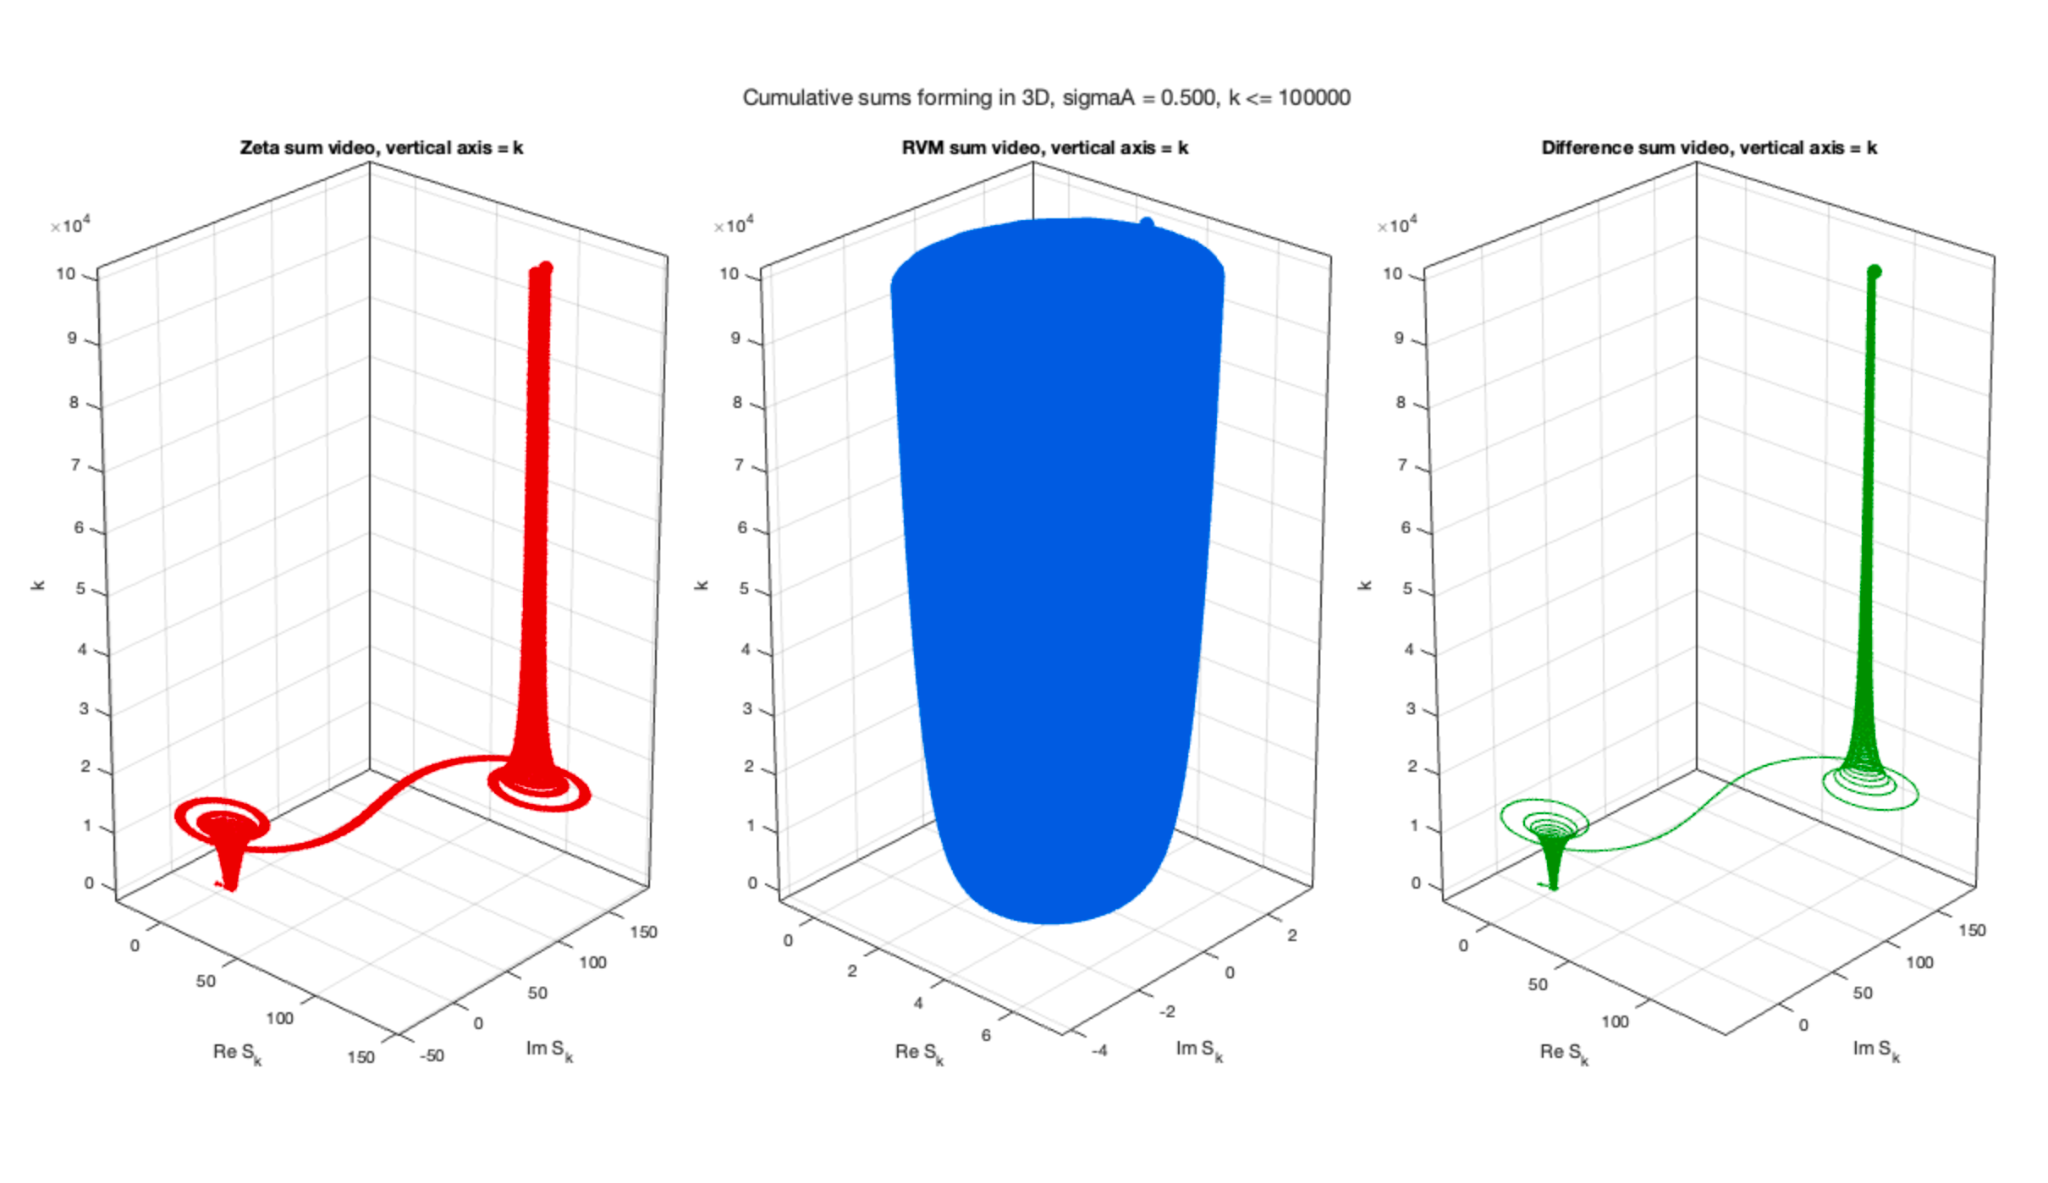
\includegraphics[width=0.95\textwidth]{fig_cumulative_3d.png}
\caption{Ordered cumulative sums for \(k\leq 100000\).  The zeta curve is the primary object; the RVM curve is a smooth control; the difference curve isolates the residual contribution.}
\label{fig:cumulative_3d}
\end{figure}

\begin{figure}[htbp]
\centering
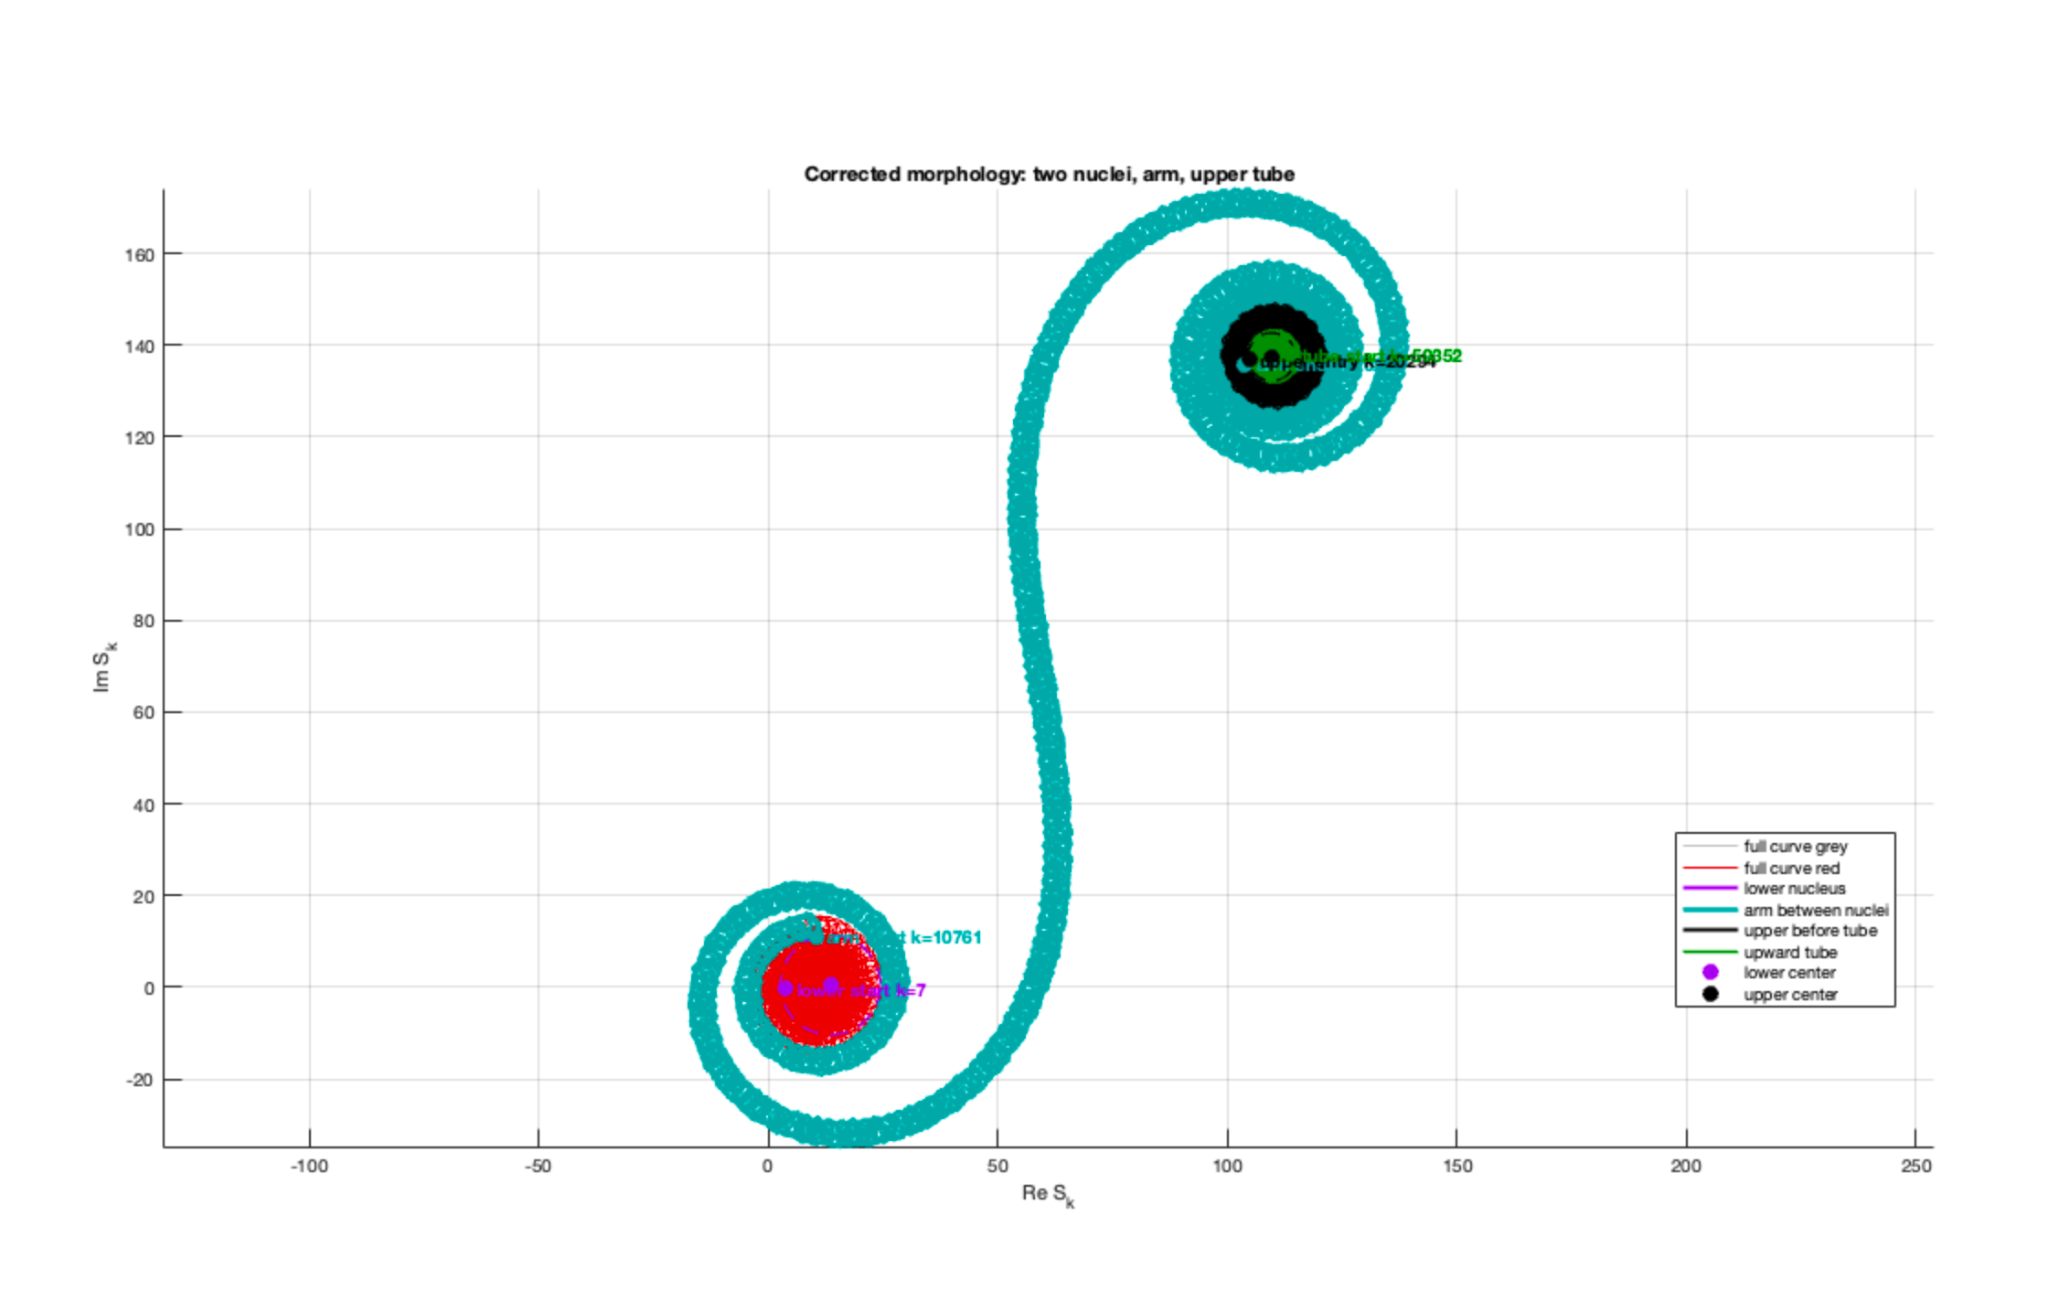
\includegraphics[width=0.95\textwidth]{fig_morphology_2d.png}
\caption{Two-dimensional morphology of the zeta cumulative curve.  The labels are descriptive finite-regime names: lower nucleus, arm, upper entry, and upper tube.}
\label{fig:morphology_2d}
\end{figure}

\begin{definition}
\label{def:descriptive_geometric_regions}
For the finite curve \(S_N^\zeta\), we use the descriptive names lower nucleus, arm, upper entry, and upper tube for the visible regions shown in Figure \ref{fig:morphology_2d}.
\end{definition}

\begin{warning}
\label{warn:finite_geometry_names}
The names in Definition \ref{def:descriptive_geometric_regions} are finite descriptive labels.  They are not asymptotic theorems.
\end{warning}

\begin{experiment}
\label{exp:final_cumulative_values}
For \(N=2000000\), the finite computation gives
\begin{align}
S_N^\zeta
&=
108.33266897301249+133.62125012982429i,
\label{eq:exp_final_zeta_value}
\\
S_N^{\RVM}
&=
1.1510041648930329-4.4564122447974022i,
\label{eq:exp_final_rvm_value}
\\
S_N^{\diff}
&=
107.1816648081158+138.07766237462528i.
\label{eq:exp_final_diff_value}
\end{align}
The corresponding moduli are
\begin{align}
|S_N^\zeta|
&=
172.01920140807934,
\label{eq:exp_final_zeta_modulus}
\\
|S_N^{\RVM}|
&=
4.6026536566617011,
\label{eq:exp_final_rvm_modulus}
\\
|S_N^{\diff}|
&=
174.79516617424036.
\label{eq:exp_final_diff_modulus}
\end{align}
The final modulus ratios are
\begin{align}
\frac{|S_N^{\RVM}|}{|S_N^\zeta|}
&=
0.026756627277572775,
\label{eq:exp_final_rvm_ratio}
\\
\frac{|S_N^{\diff}|}{|S_N^\zeta|}
&=
1.016137528505179.
\label{eq:exp_final_diff_ratio}
\end{align}
\end{experiment}

\section{Ordered window amplitudes}
\label{sec:ordered_window_amplitudes}

\begin{definition}
\label{def:window_amplitude}
For \(x\in\{\zeta,\RVM,\diff\}\), define the window amplitude
\begin{equation}
B_W^x(k)
=
\sum_{j=k}^{k+W-1}z_j^x.
\label{eq:def_window_amplitude}
\end{equation}
For \(x=\diff\), this means
\begin{equation}
B_W^{\diff}(k)
=
\sum_{j=k}^{k+W-1}d_j.
\label{eq:def_residual_window_amplitude}
\end{equation}
\end{definition}

\begin{definition}
\label{def:random_excess}
The random-walk normalized window excess is defined by
\begin{equation}
R_W^x(k)
=
\frac{|B_W^x(k)|}
{\sqrt{W}\,\rms_{j\in[k,k+W-1]}(z_j^x)}.
\label{eq:def_random_excess}
\end{equation}
\end{definition}

\begin{definition}
\label{def:window_cancellation}
The window cancellation statistic is defined by
\begin{equation}
C_W^x(k)
=
1-
\frac{|B_W^x(k)|}{\sum_{j=k}^{k+W-1}|z_j^x|}.
\label{eq:def_window_cancellation}
\end{equation}
\end{definition}

\begin{remark}
\label{rem:random_excess_interpretation}
Values \(R_W^x(k)\) of order one are compatible with a random-walk scale.  Larger values indicate stronger coherent alignment inside the ordered block.  Values \(C_W^x(k)\) close to one indicate strong cancellation, while smaller values indicate stronger internal alignment.
\end{remark}

\begin{figure}[htbp]
\centering
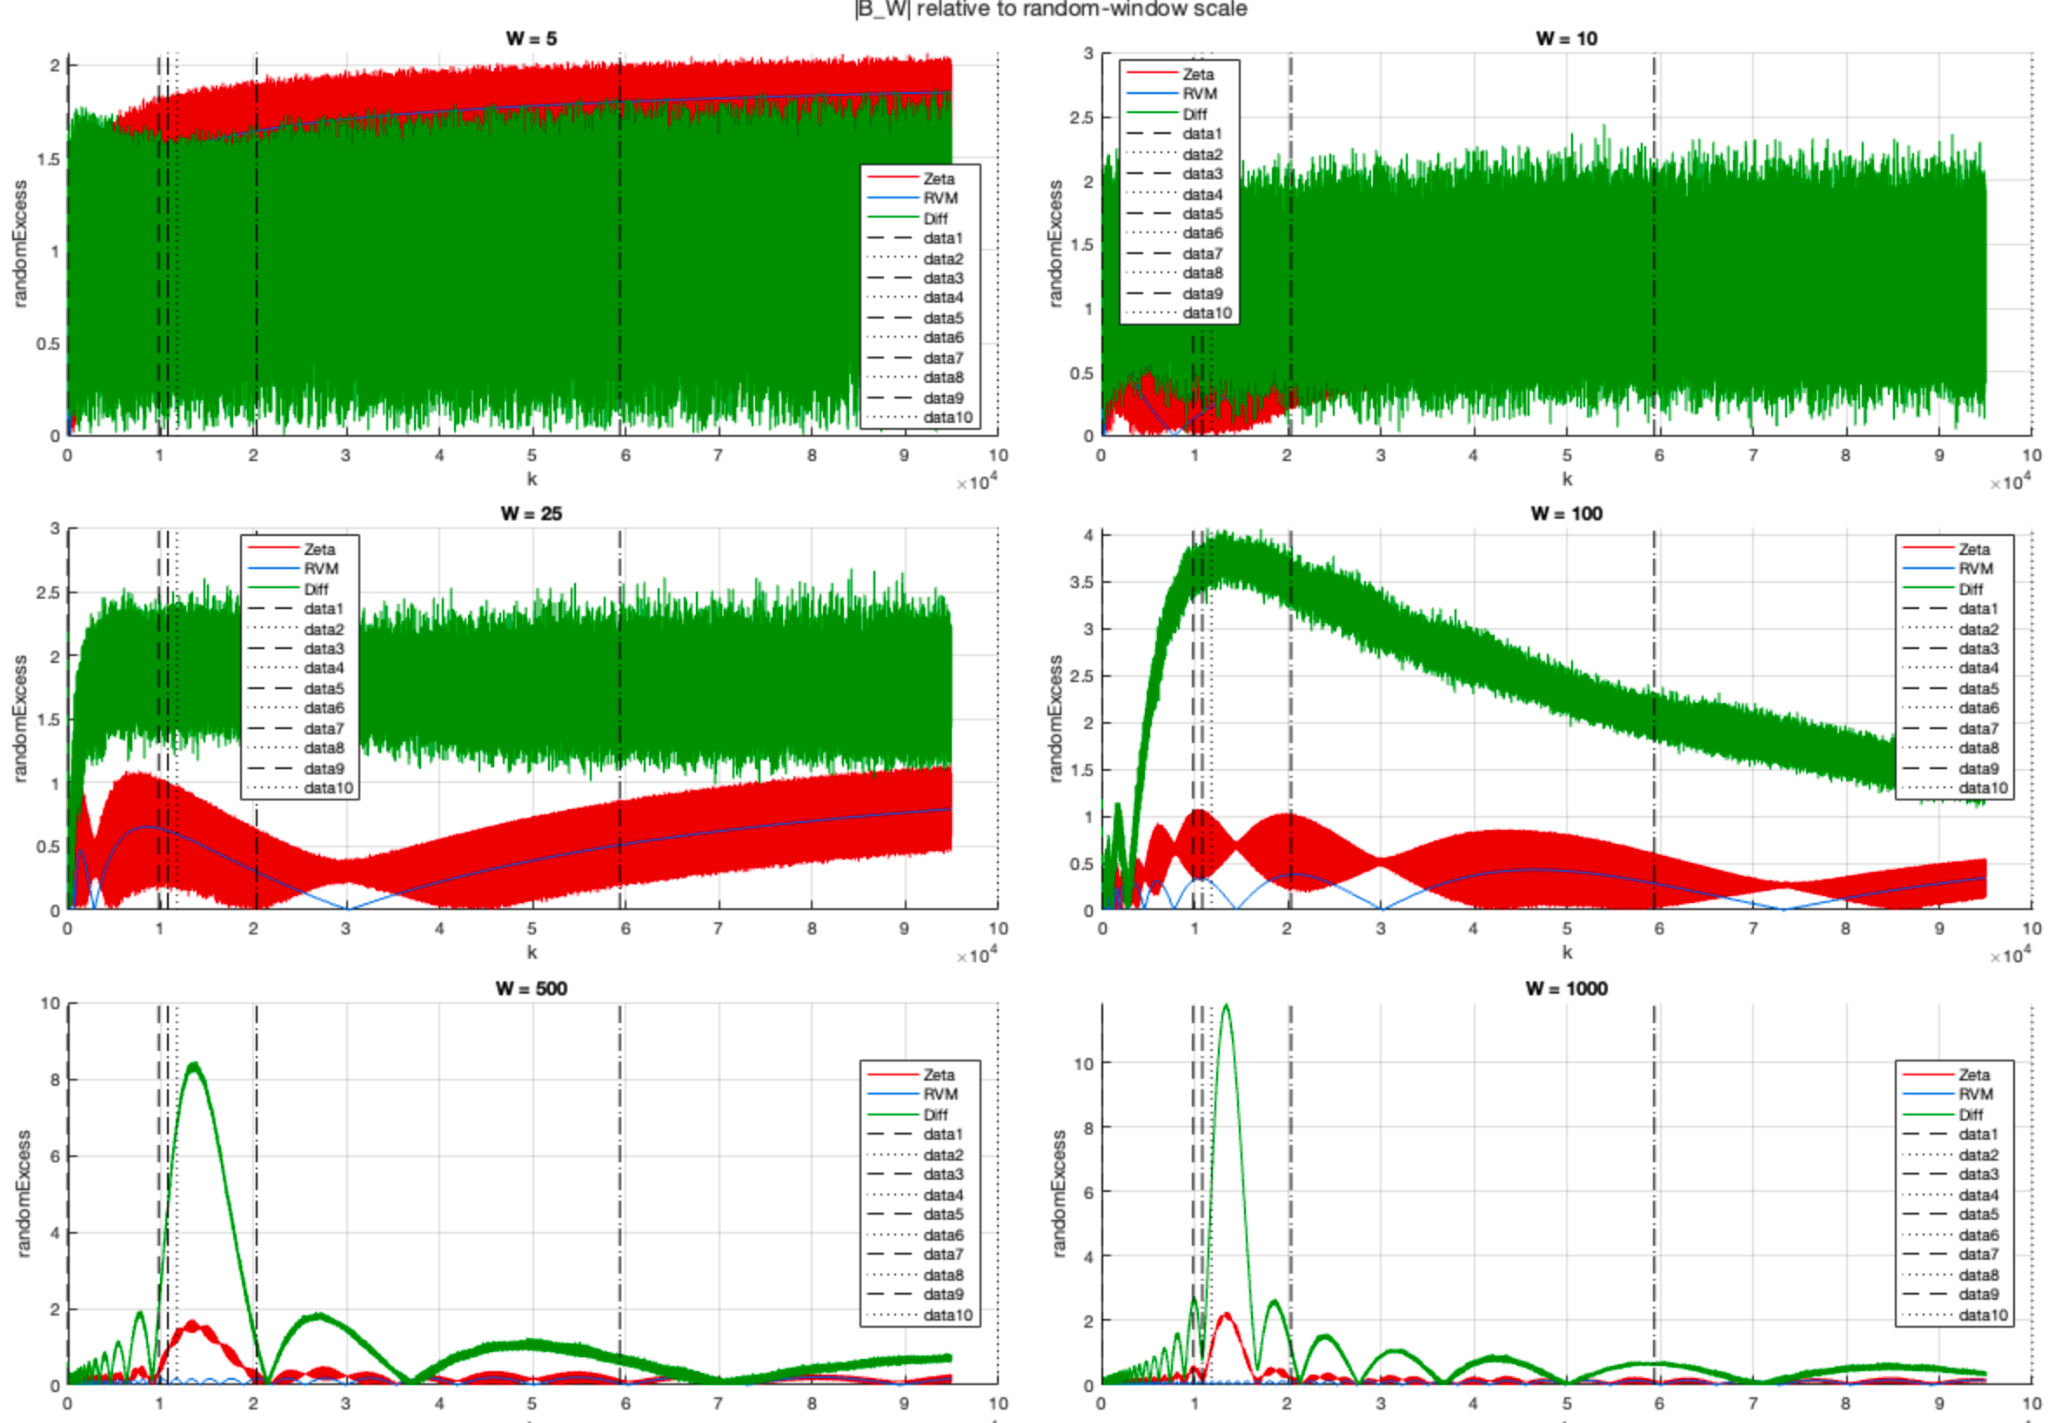
\includegraphics[width=0.98\textwidth]{fig_local_window_diag.png}
\caption{Local window diagnostics for the logarithmic proper-time transform.  The panels compare zeta, RVM/Lambert, and residual window behaviour.  The key point is that RVM is not flat: it shows the smooth susceptibility skeleton imposed by \(\tau_k\), while the zeta and residual signals excite that skeleton more strongly.}
\label{fig:local_window_diag}
\end{figure}

\begin{figure}[htbp]
\centering
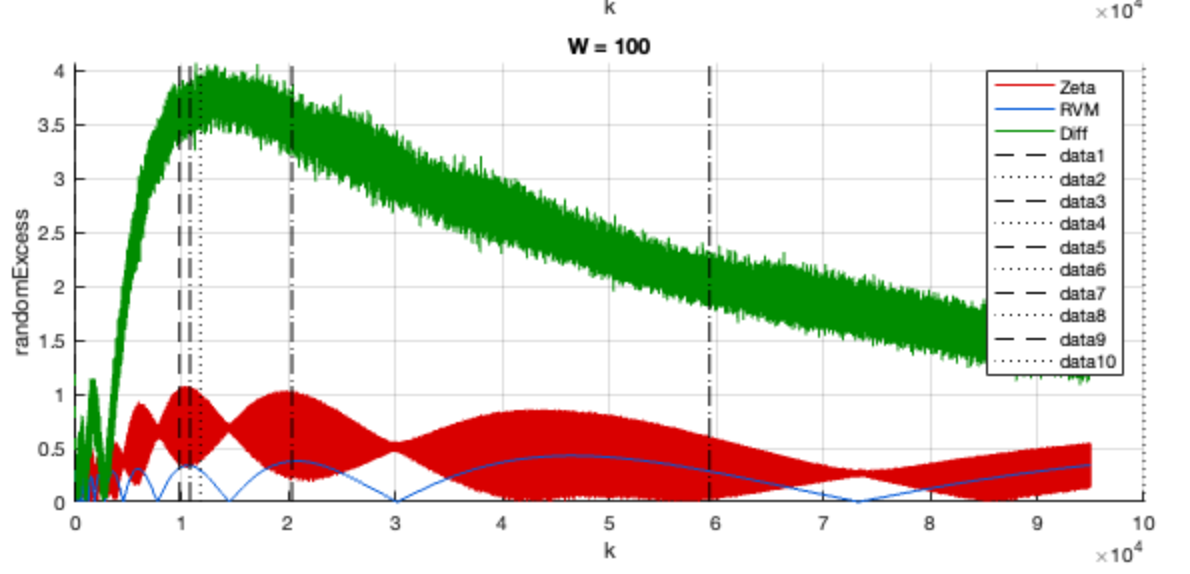
\includegraphics[width=0.95\textwidth]{fig_w100_panel.png}
\caption{The \(W=100\) window panel.  This figure resolves the early finite region where the arm begins to form.  The residual and zeta curves show stronger excitation than the RVM control.}
\label{fig:w100_panel}
\end{figure}

\begin{experiment}
\label{exp:residual_window_excess}
For the first \(N=2000000\) ordinates used in the computation, the residual window excess gives
\begin{align}
\max_k R_{500}^{\diff}(k)
&=
8.47496580076509,
\label{eq:exp_residual_window_500}
\\
\max_k R_{1000}^{\diff}(k)
&=
11.848018307196,
\label{eq:exp_residual_window_1000}
\\
\max_k R_{2000}^{\diff}(k)
&=
15.8890898166697,
\label{eq:exp_residual_window_2000}
\\
\max_k R_{5000}^{\diff}(k)
&=
11.0870615199076.
\label{eq:exp_residual_window_5000}
\end{align}
The corresponding windows lie in the finite transition region near \(k=1.3\cdot 10^4\) to \(1.5\cdot 10^4\).
\end{experiment}

\begin{experiment}
\label{exp:rvm_window_comparison}
For comparison, the RVM background gives
\begin{align}
\max_k R_{500}^{\RVM}(k)
&=
0.304008524694917,
\label{eq:exp_rvm_window_500}
\\
\max_k R_{1000}^{\RVM}(k)
&=
0.21724659866383,
\label{eq:exp_rvm_window_1000}
\\
\max_k R_{2000}^{\RVM}(k)
&=
0.156114378581857,
\label{eq:exp_rvm_window_2000}
\\
\max_k R_{5000}^{\RVM}(k)
&=
0.0988421843432245.
\label{eq:exp_rvm_window_5000}
\end{align}
\end{experiment}

\begin{heuristic}
\label{heur:block_correlation_mechanism}
This is a heuristic argument.  For any finite sequence \(z_j\), one has
\begin{equation}
|B_W(k)|^2
=
\sum_{a=0}^{W-1}\sum_{b=0}^{W-1}
z_{k+a}\overline{z_{k+b}}.
\label{eq:block_correlation_identity}
\end{equation}
Separating diagonal and off-diagonal terms gives
\begin{align}
|B_W(k)|^2
&=
\sum_{a=0}^{W-1}|z_{k+a}|^2
+
2\operatorname{Re}
\sum_{0\leq a<b\leq W-1}z_{k+a}\overline{z_{k+b}}.
\label{eq:block_correlation_offdiagonal}
\end{align}
The diagonal part sets the random-walk scale.  The off-diagonal part determines whether the ordered block is coherently enhanced or suppressed.  In the present transform, the phase differences are
\begin{equation}
\theta_{k+a}^\zeta-\theta_{k+b}^\zeta
=
\gamma_{k+a}\tau_{k+a}-\gamma_{k+b}\tau_{k+b}.
\label{eq:block_phase_difference}
\end{equation}
Thus the window excess probes ordered phase correlations of the logarithmic proper-time field.
\end{heuristic}

\section{Phase portraits and local drift}
\label{sec:phase_portraits_local_drift}

\begin{figure}[H]
\centering
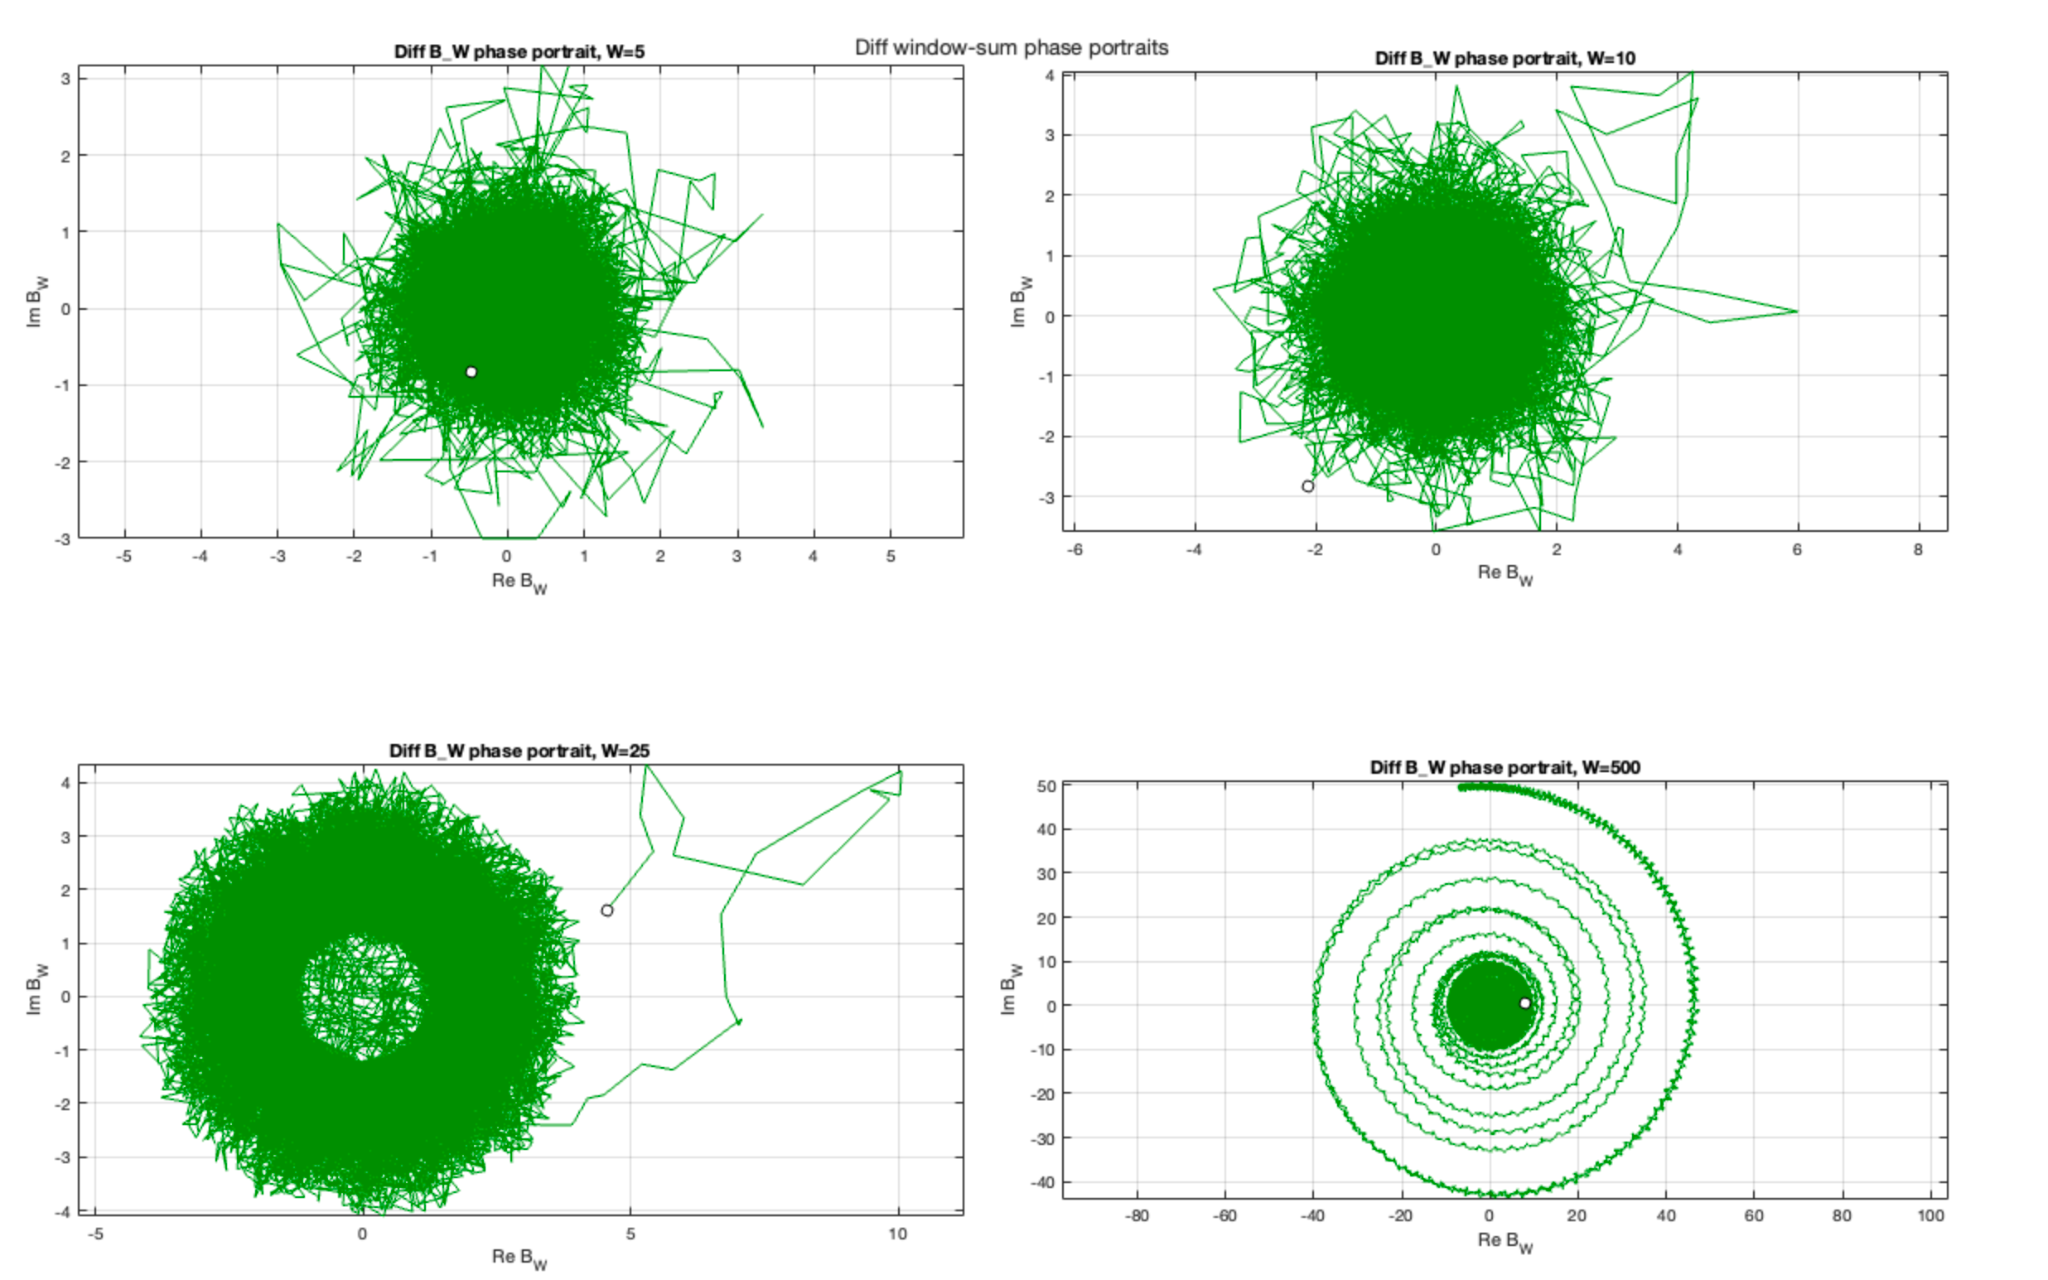
\includegraphics[width=0.88\textwidth]{fig_phase_portraits_diff.png}
\caption{Phase portraits and local drift for selected window sums.  The residual windows form organized loops rather than featureless scatter, and the local drift concentrates near the same finite transition region identified by the window diagnostics.}
\label{fig:phase_portraits_diff}
\end{figure}
\vspace{-0.15cm}

\begin{remark}
\label{rem:phase_portraits_role}
The phase portraits are not independent assumptions.  They are local projections of the same ordered window amplitudes defined in \eqref{eq:def_window_amplitude}.  Their role is to show that the residual sequence is not featureless after ordered summation.
\end{remark}

\section{Nearest-neighbor gaps of the transformed function}
\label{sec:nearest_neighbor_gaps}

\begin{definition}
\label{def:direct_vector_gaps}
The direct vector gaps of the transformed zeta and RVM terms are
\begin{align}
D_k^\zeta
&=
|z_{k+1}^\zeta-z_k^\zeta|,
\label{eq:def_zeta_vector_gap}
\\
D_k^{\RVM}
&=
|z_{k+1}^{\RVM}-z_k^{\RVM}|.
\label{eq:def_rvm_vector_gap}
\end{align}
The residual vector gap is
\begin{equation}
D_k^{\diff}
=
|d_{k+1}-d_k|.
\label{eq:def_diff_vector_gap}
\end{equation}
\end{definition}

\begin{definition}
\label{def:functional_angular_gaps}
The angular functional gaps are
\begin{align}
\Delta\theta_k^\zeta
&=
\gamma_{k+1}\tau_{k+1}-\gamma_k\tau_k,
\label{eq:def_zeta_functional_gap}
\\
\Delta\theta_k^{\RVM}
&=
\gamma_{k+1}^{\RVM}\tau_{k+1}-\gamma_k^{\RVM}\tau_k,
\label{eq:def_rvm_functional_gap}
\\
\Delta\theta_k^{\rm resid}
&=
\Delta\theta_k^\zeta-\Delta\theta_k^{\RVM}.
\label{eq:def_resid_functional_gap}
\end{align}
\end{definition}

\begin{definition}
\label{def:locally_unfolded_functional_gap}
For a local unfolding window \(W_{\rm norm}=2000\), define
\begin{align}
s_k^{\rm func,\zeta}
&=
\frac{\Delta\theta_k^\zeta}
{\operatorname{movmedian}(\Delta\theta^\zeta,W_{\rm norm})},
\label{eq:def_sfunc_zeta}
\\
s_k^{\rm func,\RVM}
&=
\frac{\Delta\theta_k^{\RVM}}
{\operatorname{movmedian}(\Delta\theta^{\RVM},W_{\rm norm})}.
\label{eq:def_sfunc_rvm}
\end{align}
\end{definition}

\begin{figure}[htbp]
\centering
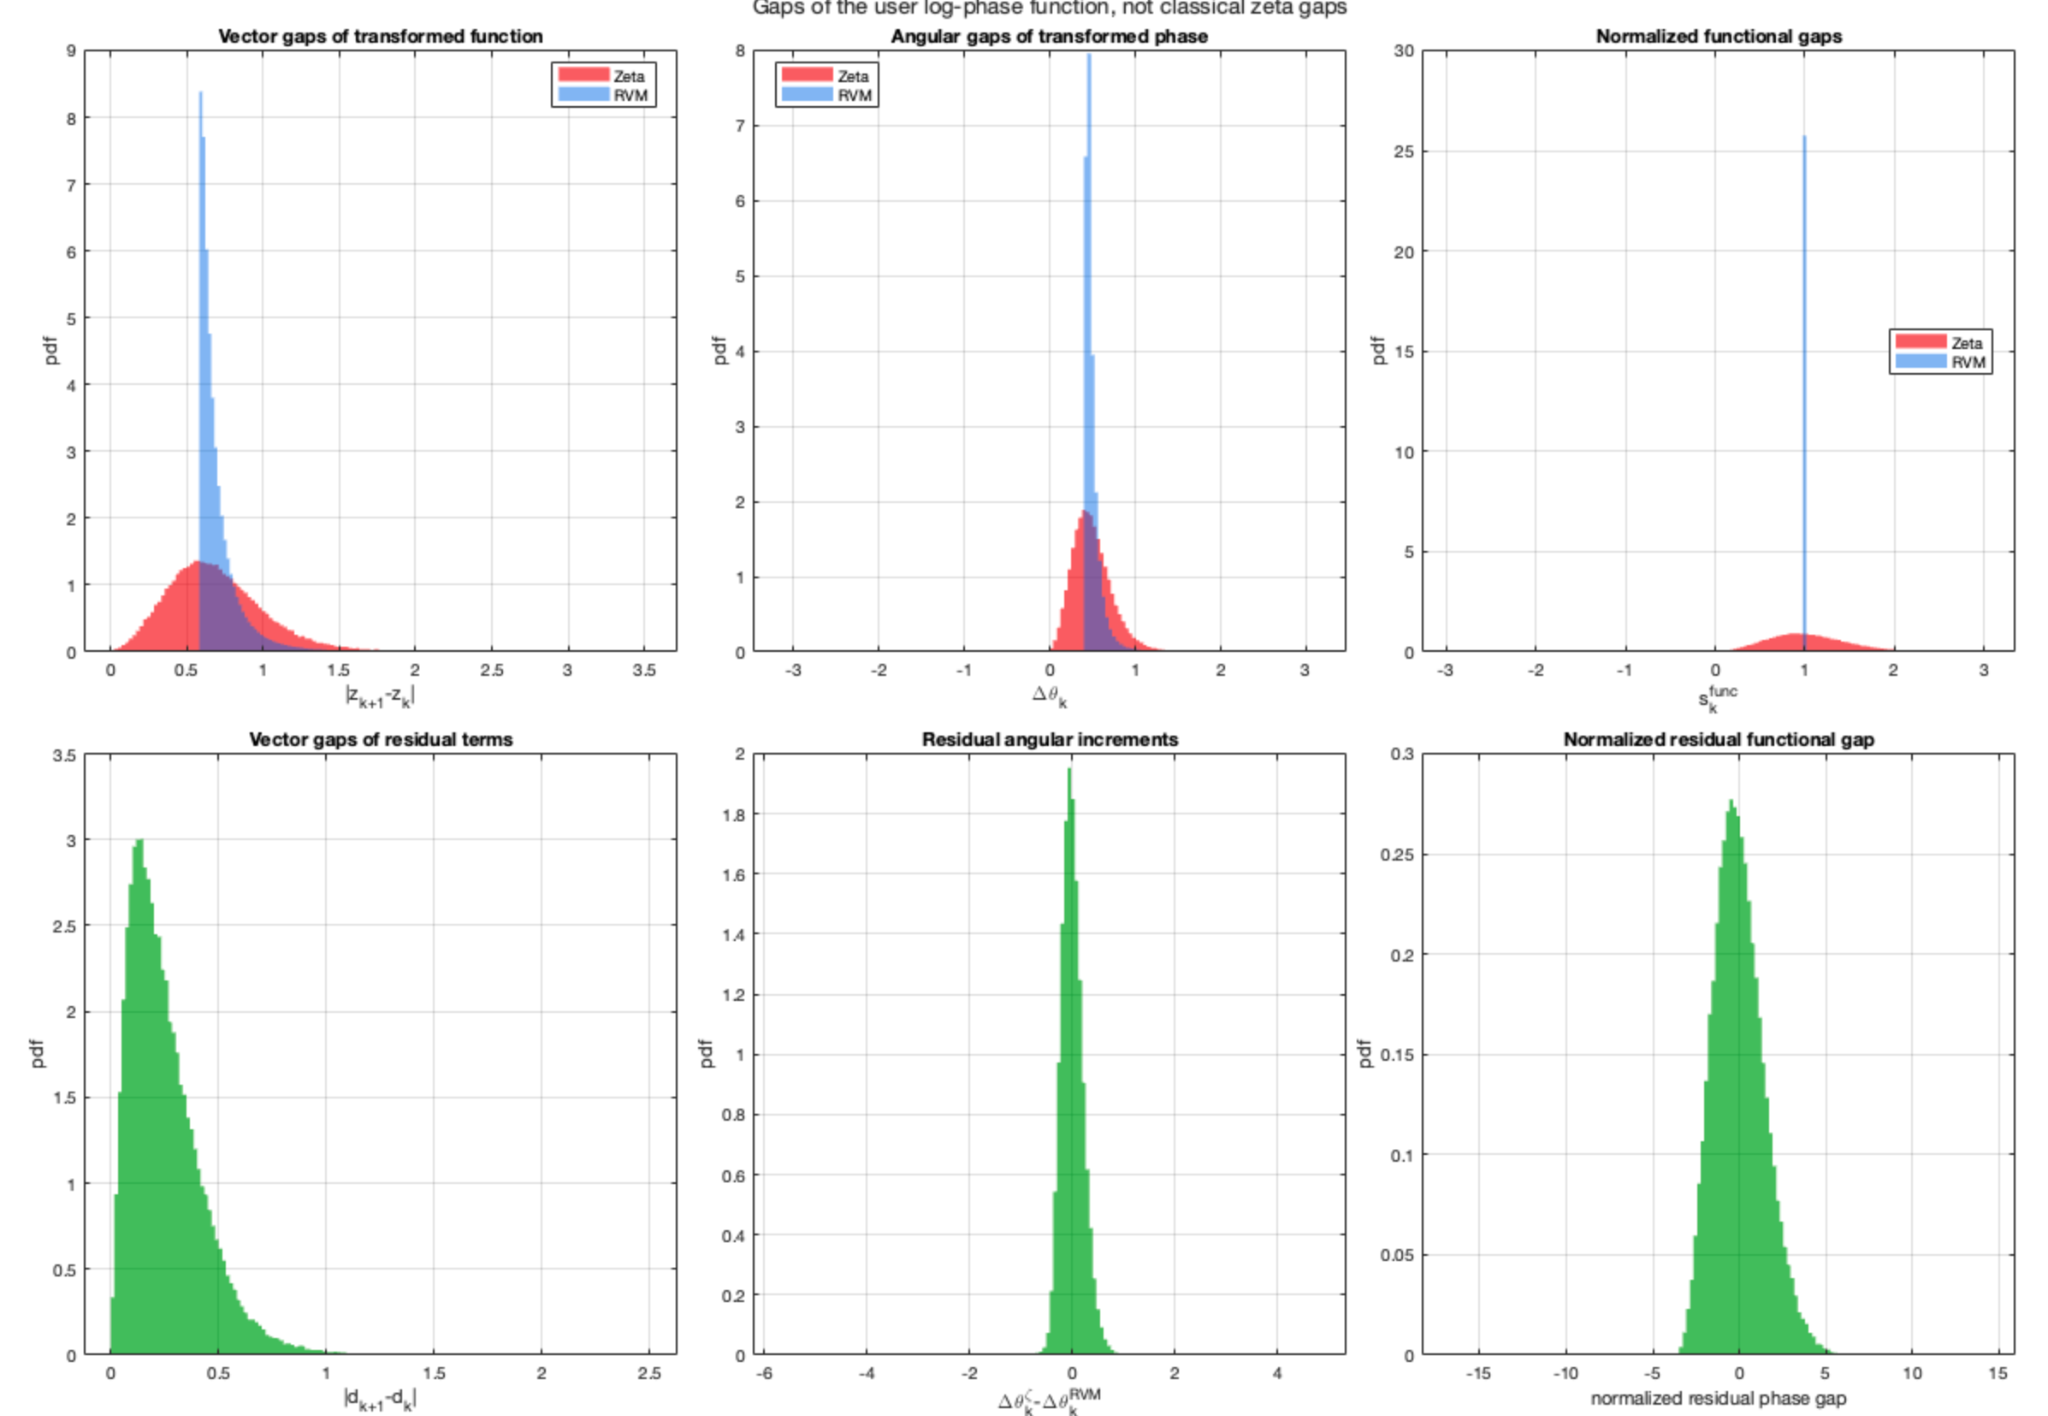
\includegraphics[width=0.95\textwidth]{fig_functional_gaps.png}
\caption{Nearest-neighbor gap diagnostics for the transformed function.  The zeta functional gaps are much broader than the RVM control, while the residual one-step vector gap has its own radial law.}
\label{fig:functional_gaps}
\end{figure}

\begin{experiment}
\label{exp:functional_gap_statistics}
For \(N=100000\) and \(W_{\rm norm}=2000\), the direct vector-gap statistics include
\begin{align}
\mean(D^\zeta)
&=
0.6996727187446995,
\label{eq:exp_mean_dzeta}
\\
\mean(D^{\RVM})
&=
0.70476664009997447,
\label{eq:exp_mean_drvm}
\\
\mean(D^{\diff})
&=
0.25693458832515564.
\label{eq:exp_mean_ddiff}
\end{align}
The standard deviations are
\begin{align}
\operatorname{std}(D^\zeta)
&=
0.33739092323816883,
\label{eq:exp_std_dzeta}
\\
\operatorname{std}(D^{\RVM})
&=
0.1720230232135381,
\label{eq:exp_std_drvm}
\\
\operatorname{std}(D^{\diff})
&=
0.17544139070373949.
\label{eq:exp_std_ddiff}
\end{align}
For the locally normalized functional angular gaps,
\begin{align}
\operatorname{std}(s^{\rm func,\zeta})
&=
0.4470387560827801,
\label{eq:exp_std_sfunc_zeta}
\\
\operatorname{std}(s^{\rm func,\RVM})
&=
0.044621414720808834.
\label{eq:exp_std_sfunc_rvm}
\end{align}
Thus the zeta functional gaps have approximately ten times the standard deviation of the RVM control after local normalization.
\end{experiment}

\section{Rayleigh local residual gaps}
\label{sec:rayleigh_local_residual_gaps}

\begin{definition}
\label{def:mean_normalized_diff_gap}
The mean-normalized residual vector gap is
\begin{equation}
s_k^{\rm diffvec}
=
\frac{|d_{k+1}-d_k|}{\mean_j |d_{j+1}-d_j|}.
\label{eq:def_mean_normalized_diff_gap}
\end{equation}
\end{definition}

\begin{definition}
\label{def:comparison_laws}
The comparison laws used in the nearest-neighbor residual test are
\begin{align}
p_{\GUE}(s)
&=
\frac{32}{\pi^2}s^2e^{-4s^2/\pi},
\label{eq:def_gue_wigner_surmise}
\\
p_{\Poisson}(s)
&=
e^{-s},
\label{eq:def_poisson_law}
\\
p_{\Rayleigh}(s)
&=
\frac{s}{\sigma_R^2}
\exp\left(-\frac{s^2}{2\sigma_R^2}\right),
\qquad
\sigma_R=\sqrt{\frac{2}{\pi}}.
\label{eq:def_rayleigh_law}
\end{align}
\end{definition}

\begin{figure}[H]
\centering
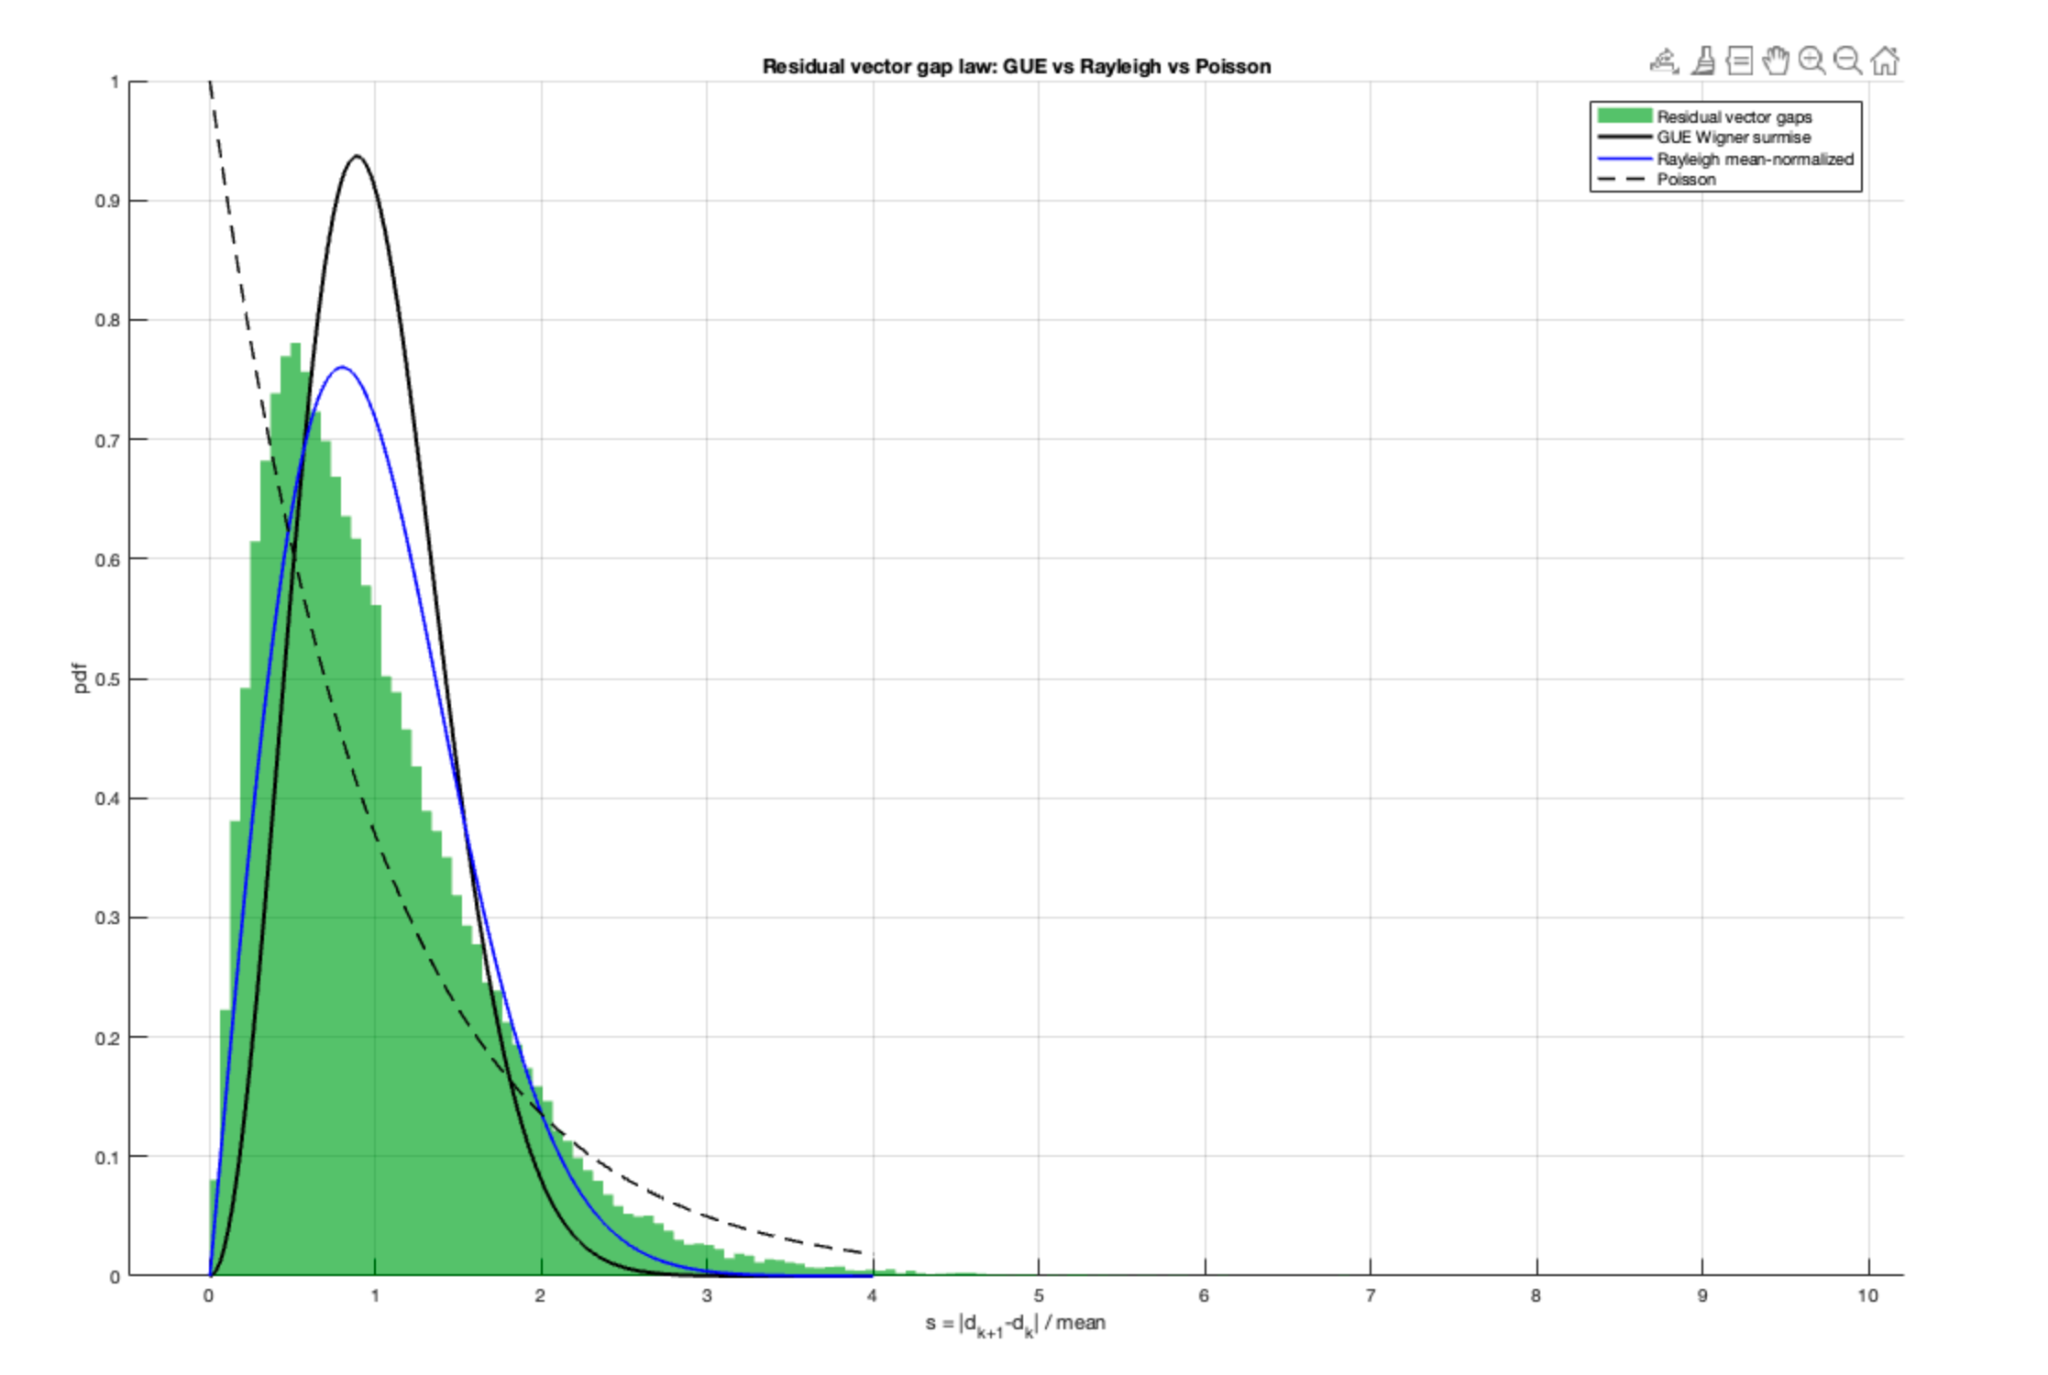
\includegraphics[width=0.84\textwidth]{fig_rayleigh_gap_law.png}
\caption{Nearest-neighbor residual vector gaps of the transformed function.  After normalization by their mean, the residual gaps \(|d_{k+1}-d_k|\) are compared with the GUE Wigner surmise, Poisson spacing, and the mean-normalized Rayleigh law.}
\label{fig:rayleigh_gap_law}
\end{figure}
\vspace{-0.15cm}

\begin{experiment}
\label{exp:rayleigh_gap_law}
For \(N=100000\), the mean raw residual vector gap is
\begin{equation}
\mean_k |d_{k+1}-d_k|
=
0.25693458832515564,
\label{eq:exp_mean_raw_diff_gap}
\end{equation}
and the median normalized residual vector gap is
\begin{equation}
\median(s^{\rm diffvec})
=
0.84934875093822626.
\label{eq:exp_median_normalized_diff_gap}
\end{equation}
The Kolmogorov--Smirnov distances are
\begin{align}
\KS_{\GUE}
&=
0.27524262614727296,
\label{eq:exp_ks_gue}
\\
\KS_{\Rayleigh}
&=
0.083901339184571433,
\label{eq:exp_ks_rayleigh}
\\
\KS_{\Poisson}
&=
0.15549638718785452.
\label{eq:exp_ks_poisson}
\end{align}
The near-zero CDF exponent, fitted from
\begin{equation}
P(s\leq \varepsilon)
\sim
\varepsilon^\alpha,
\label{eq:exp_near_zero_cdf_law}
\end{equation}
is
\begin{equation}
\alpha
=
1.9625998029380822.
\label{eq:exp_near_zero_cdf_exponent}
\end{equation}
\end{experiment}

\begin{remark}
\label{rem:local_rayleigh_not_gue}
The value \eqref{eq:exp_near_zero_cdf_exponent} is close to the Rayleigh CDF exponent \(2\), not to the GUE nearest-neighbor exponent \(3\), and not to the Poisson exponent \(1\).  Thus the one-step residual vector gaps are Rayleigh-like, not GUE-like.
\end{remark}

\begin{heuristic}
\label{heur:planar_fluctuation}
This is a heuristic interpretation.  The residual difference \(d_{k+1}-d_k\) is a complex planar quantity.  If its real and imaginary components behave approximately as centered Gaussian components at the one-step level, then its modulus is expected to follow a Rayleigh-type radial law.  Experiment \ref{exp:rayleigh_gap_law} is consistent with this interpretation.
\end{heuristic}

\section{Effective logarithmic redshift}
\label{sec:effective_logarithmic_redshift}

\begin{heuristic}
\label{heur:scale_redshift}
This is a heuristic interpretation.  Introduce the scale coordinate
\begin{equation}
u
=
\log k.
\label{eq:scale_coordinate_u}
\end{equation}
Then the logarithmic proper time in \eqref{eq:def_logarithmic_proper_time} becomes
\begin{equation}
\tau_k
=
\pi\frac{\log u}{u}.
\label{eq:proper_time_scale_coordinate}
\end{equation}
Formally, this may be read as an effective redshift factor
\begin{equation}
d\tau
=
\sqrt{-g_{tt}(u)}\,dt,
\qquad
\sqrt{-g_{tt}(u)}
=
\pi\frac{\log u}{u}.
\label{eq:effective_redshift_factor}
\end{equation}
Equivalently, one may write the scale-metric ansatz
\begin{equation}
ds^2
=
-\pi^2\frac{(\log u)^2}{u^2}dt^2+du^2.
\label{eq:effective_scale_metric}
\end{equation}
\end{heuristic}

\begin{warning}
\label{warn:not_physical_metric}
Equation \eqref{eq:effective_scale_metric} is not asserted to be a physical spacetime metric.  It is an effective scale-metric interpretation of the logarithmic clock in the spectral observable.
\end{warning}

\section{Finite computational proposition}
\label{sec:finite_computational_proposition}

\begin{proposition}
\label{prop:finite_residual_window_excess}
For the first \(N=2000000\) ordinates in the finite computation, with \(\tau_k\) as in Definition \ref{def:logarithmic_proper_time}, the residual window excess satisfies
\begin{align}
\max_k R_{500}^{\diff}(k)
&>
8,
\label{eq:prop_residual_excess_500_bound}
\\
\max_k R_{1000}^{\diff}(k)
&>
11,
\label{eq:prop_residual_excess_1000_bound}
\\
\max_k R_{2000}^{\diff}(k)
&>
15.
\label{eq:prop_residual_excess_2000_bound}
\end{align}
\end{proposition}

\begin{proof}
The finite numerical values in Experiment \ref{exp:residual_window_excess} give
\begin{align}
\max_k R_{500}^{\diff}(k)
&=
8.47496580076509,
\label{eq:proof_prop_500_exact}
\\
\max_k R_{1000}^{\diff}(k)
&=
11.848018307196,
\label{eq:proof_prop_1000_exact}
\\
\max_k R_{2000}^{\diff}(k)
&=
15.8890898166697.
\label{eq:proof_prop_2000_exact}
\end{align}
These finite values imply \eqref{eq:prop_residual_excess_500_bound}, \eqref{eq:prop_residual_excess_1000_bound}, and \eqref{eq:prop_residual_excess_2000_bound}.
\end{proof}

\begin{question}
\label{ques:persistence_further_transitions}
The computation up to \(N=2000000\) shows a stabilized upper-tube regime after the early transitions.  Do further phase-block reorganizations occur at larger heights, producing new arms, tubes, or relocations of the cumulative geometry?
\end{question}




\section{Counting-coordinate balance and off-critical detection}
\label{sec:counting_coordinate_balance_offcritical_detection}

The logarithmic proper-time observable studied in the preceding sections uses the ordinate coordinate \(\gamma_k\).  It detects ordered phase geometry along the vertical direction of the zero set.  This section records a second, independent construction involving the real coordinate \(\sigma_k\).  Its role is different: it is a signed detector of displacement away from the critical line.

\begin{warning}
\label{warn:dx_status}

The material in this section is a formal finite construction based on the completed zeta function, local normalization at zeros, and the counting coordinate.  It is not used as a proof of the Riemann Hypothesis.  It records what the balance quantity detects in the two alternatives \(\sigma_k=1/2\) and \(\sigma_k\neq1/2\).

\end{warning}

\subsection{Completed zeta function and the real symmetry}
\label{subsec:completed_zeta_real_symmetry}

\begin{definition}
\label{def:completed_zeta_xi}

The completed zeta function is
\begin{equation}
\xi(s)
=
\frac{1}{2}s(s-1)\pi^{-s/2}\Gamma\left(\frac{s}{2}\right)\zeta(s).
\label{eq:completed_zeta_xi}
\end{equation}
It satisfies the functional equation
\begin{equation}
\xi(s)=\xi(1-s).
\label{eq:completed_zeta_functional_equation}
\end{equation}

\end{definition}

\begin{lemma}
\label{lem:xi_modulus_symmetry}

For real \(\sigma\) and real \(\gamma\), one has
\begin{equation}
|\xi(\sigma+i\gamma)|
=
|\xi(1-\sigma+i\gamma)|.
\label{eq:xi_modulus_symmetry}
\end{equation}

\end{lemma}

\begin{proof}
Since \(\xi\) is real on the real axis, it satisfies
\begin{equation}
\xi(\overline{s})=\overline{\xi(s)}.
\label{eq:xi_real_on_real_axis_symmetry}
\end{equation}
Using \eqref{eq:completed_zeta_functional_equation}, one obtains
\begin{align}
\xi(1-\sigma+i\gamma)
&=
\overline{\xi(1-\sigma-i\gamma)}
\label{eq:xi_modulus_symmetry_proof_first}
\\
&=
\overline{\xi(\sigma+i\gamma)}.
\label{eq:xi_modulus_symmetry_proof_second}
\end{align}
Taking absolute values gives \eqref{eq:xi_modulus_symmetry}.
\end{proof}

\subsection{Zeros and local normalization}
\label{subsec:zeros_local_normalization}

\begin{definition}
\label{def:general_nontrivial_zero}

Let
\begin{equation}
\rho_k
=
\sigma_k+i\gamma_k
\label{eq:general_nontrivial_zero}
\end{equation}
denote the nontrivial zeros of \(\zeta(s)\), ordered by nondecreasing positive ordinate and counted with multiplicity.  Under RH, one has \(\sigma_k=1/2\) for all nontrivial zeros.

\end{definition}

\begin{definition}
\label{def:real_displacement_from_critical_line}

For a real parameter \(\beta\), define the displacement from the critical line by
\begin{equation}
\delta
=
\beta-\frac{1}{2}.
\label{eq:real_displacement_from_critical_line}
\end{equation}
At a zero \(\rho_k=\sigma_k+i\gamma_k\), the corresponding displacement is
\begin{equation}
\delta_k
=
\sigma_k-\frac{1}{2}.
\label{eq:zero_real_displacement_from_critical_line}
\end{equation}

\end{definition}

\begin{lemma}
\label{lem:local_normalization_at_simple_zero}

Assume that \(\rho_k\) is a simple zero of \(\xi\).  For \(\delta\neq0\), define
\begin{equation}
A_k(\delta)
=
\frac{\xi(\rho_k+\delta)}{\delta\,\xi'(\rho_k)}.
\label{eq:local_normalization_Ak}
\end{equation}
Then
\begin{equation}
\lim_{\delta\to0}A_k(\delta)=1.
\label{eq:local_normalization_Ak_limit}
\end{equation}

\end{lemma}

\begin{proof}
Since \(\xi\) is entire and \(\rho_k\) is a simple zero, one has
\begin{equation}
\xi(\rho_k)=0,
\qquad
\xi'(\rho_k)\neq0.
\label{eq:simple_zero_conditions_xi}
\end{equation}
Taylor expansion gives
\begin{equation}
\xi(\rho_k+\delta)
=
\delta\xi'(\rho_k)+O(\delta^2)
\label{eq:xi_taylor_at_simple_zero}
\end{equation}
as \(\delta\to0\).  Dividing by \(\delta\xi'(\rho_k)\) gives \eqref{eq:local_normalization_Ak_limit}.
\end{proof}

\begin{definition}
\label{def:Ck_delta_coefficient}

Assume that \(\rho_k\) is simple.  For \(\delta\neq0\), define
\begin{equation}
C_k(\delta)
=
\left|
\frac{\xi(\rho_k+\delta)}{\delta\,\xi'(\rho_k)}
\right|^{-2},
\label{eq:Ck_delta_coefficient}
\end{equation}
whenever the expression is defined.

\end{definition}

\begin{lemma}
\label{lem:Ck_delta_positive}

Whenever \(C_k(\delta)\) is defined, one has
\begin{equation}
C_k(\delta)>0.
\label{eq:Ck_delta_positive}
\end{equation}

\end{lemma}

\begin{proof}
The denominator in \eqref{eq:Ck_delta_coefficient} is nonzero for a simple zero and \(\delta\neq0\).  The definition is used only when the numerator is nonzero.  Hence the quotient has positive modulus, and its inverse square is a positive real number.
\end{proof}

\subsection{Counting coordinate}
\label{subsec:counting_coordinate}

\begin{definition}
\label{def:zero_counting_function}

Let
\begin{equation}
N(T)
=
\#\{k:0<\gamma_k\leq T\}
\label{eq:zero_counting_function}
\end{equation}
be the zero-counting function.

\end{definition}

\begin{theorem}[Riemann--von Mangoldt]
\label{thm:riemann_von_mangoldt_counting}

As \(T\to\infty\),
\begin{equation}
N(T)
=
\frac{T}{2\pi}\log\frac{T}{2\pi}
-
\frac{T}{2\pi}
+
O(\log T).
\label{eq:riemann_von_mangoldt_counting}
\end{equation}

\end{theorem}

\begin{proof}
This is the classical Riemann--von Mangoldt counting formula; see \cite{Titchmarsh1986,Edwards2001,IwaniecKowalski2004}.
\end{proof}

\begin{lemma}
\label{lem:N_gamma_k_equals_k}

With the ordering convention of Definition \ref{def:general_nontrivial_zero}, one has
\begin{equation}
N(\gamma_k)=k.
\label{eq:N_gamma_k_equals_k}
\end{equation}

\end{lemma}

\begin{proof}
By definition, \(N(\gamma_k)\) counts the nontrivial zeros with positive ordinate not exceeding \(\gamma_k\), counted with multiplicity.  Under the ordering convention, this number is \(k\).
\end{proof}

\begin{definition}
\label{def:logarithmic_counting_coordinate_Dx}

At a zero ordinate \(\gamma_k\), define the logarithmic counting coordinate
\begin{equation}
u_k
=
\log N(\gamma_k)
=
\log k.
\label{eq:logarithmic_counting_coordinate_Dx}
\end{equation}

\end{definition}

\subsection{The finite balance quantity \texorpdfstring{\(D_X\)}{D_X}}
\label{subsec:finite_balance_quantity_DX}

\begin{definition}
\label{def:DX_beta_balance}

For \(X>0\) and real \(\beta\), set \(\delta=\beta-1/2\) and define
\begin{equation}
D_X(\beta)
=
\sum_{\gamma_k\leq X}
C_k(\delta)
\left(
N(\gamma_k)^{2\delta}
-
N(\gamma_k)^{-2\delta}
\right).
\label{eq:DX_beta_balance}
\end{equation}
Equivalently, using Lemma \ref{lem:N_gamma_k_equals_k},
\begin{equation}
D_X(\beta)
=
\sum_{k\leq N(X)}
C_k(\delta)
\left(
k^{2\delta}-k^{-2\delta}
\right).
\label{eq:DX_beta_indexed_balance}
\end{equation}

\end{definition}

\begin{lemma}
\label{lem:DX_sinh_form}

The summand in \eqref{eq:DX_beta_indexed_balance} can be written as
\begin{equation}
k^{2\delta}-k^{-2\delta}
=
e^{2\delta u_k}-e^{-2\delta u_k}
=
2\sinh(2\delta u_k),
\qquad
u_k=\log k.
\label{eq:DX_sinh_form}
\end{equation}

\end{lemma}

\begin{proof}
Substitute \(u_k=\log k\) into \(k^{2\delta}=e^{2\delta\log k}\) and \(k^{-2\delta}=e^{-2\delta\log k}\).
\end{proof}

\begin{remark}
\label{rem:Dx_is_one_sided}

The quantity \(D_X(\beta)\) is one-sided in the real displacement parameter.  It compares the two weights attached to \(+\delta\) and \(-\delta\), but it is evaluated on the same positive counting coordinate \(u_k=\log k\).  Therefore the actual counting coordinate is not transformed into its negative.

\end{remark}

\subsection{Critical involution: what changes and what does not}
\label{subsec:critical_involution_what_changes}

\begin{lemma}
\label{lem:critical_involution_changes_delta_not_u}

Under the critical involution \(s\mapsto1-s\), the real displacement changes sign,
\begin{equation}
\delta
=
\beta-\frac{1}{2}
\longmapsto
-
\delta,
\label{eq:critical_involution_changes_delta}
\end{equation}
while the positive counting coordinate attached to the ordinate remains
\begin{equation}
u_k
=
\log N(\gamma_k)
=
\log k
>
0
\qquad
(k>1).
\label{eq:critical_involution_u_stays_positive}
\end{equation}
Consequently, the critical involution exchanges the two weights by changing the sign of \(\delta\), not by changing the actual coordinate \(u_k\) into \(-u_k\):
\begin{equation}
e^{2\delta u_k}
\longleftrightarrow
e^{-2\delta u_k}.
\label{eq:critical_involution_weight_exchange_corrected}
\end{equation}

\end{lemma}

\begin{proof}
If \(s=\beta+i\gamma\), then \(1-s=1-\beta-i\gamma\).  The real displacement from the critical line is \(\delta=\beta-1/2\), and after the involution it becomes \(-\delta\).  The coordinate \(u_k\) is defined from the counting index of the ordinate and remains the positive number \(\log k\).  Substituting \(\delta\) and \(-\delta\) into \(e^{2\delta u_k}\) gives the exchange in \eqref{eq:critical_involution_weight_exchange_corrected}.
\end{proof}

\begin{warning}
\label{warn:not_u_equals_minus_u}

It is not correct to identify the actual counting coordinate with the transformation \(u_k\mapsto -u_k\).  The equality \(u_k=-u_k\) would force \(u_k=0\), which is not the case for \(k>1\).  The correct statement is the weight exchange
\begin{equation}
e^{2\delta u_k}
\leftrightarrow
e^{-2\delta u_k}
\label{eq:not_u_equals_minus_u_weight_exchange}
\end{equation}
caused by \(\delta\mapsto-\delta\) at fixed positive \(u_k\).  One may introduce a formal auxiliary signed coordinate to describe the completed pair of weights, but that auxiliary notation is not the physical counting coordinate \(u_k=\log k\).

\end{warning}

\begin{lemma}
\label{lem:analytic_symmetry_counting_weight_exchange}

The functional equation gives the analytic symmetry
\begin{equation}
|\xi(\beta+i\gamma)|
=
|\xi(1-\beta+i\gamma)|,
\label{eq:analytic_symmetry_beta_gamma}
\end{equation}
while the counting construction gives the weight exchange
\begin{equation}
N(\gamma_k)^{2(\beta-1/2)}
\longleftrightarrow
N(\gamma_k)^{-2(\beta-1/2)}.
\label{eq:counting_weight_exchange_beta_gamma}
\end{equation}

\end{lemma}

\begin{proof}
Equation \eqref{eq:analytic_symmetry_beta_gamma} is Lemma \ref{lem:xi_modulus_symmetry}.  Equation \eqref{eq:counting_weight_exchange_beta_gamma} follows from Lemma \ref{lem:critical_involution_changes_delta_not_u} with \(u_k=\log N(\gamma_k)\).
\end{proof}

\begin{lemma}
\label{lem:completed_pair_cancellation_corrected}

For each fixed \(k\), the completed formal pair of opposite real displacements cancels algebraically:
\begin{equation}
\left(e^{2\delta u_k}-e^{-2\delta u_k}\right)
+
\left(e^{-2\delta u_k}-e^{2\delta u_k}\right)
=
0.
\label{eq:completed_pair_cancellation_corrected}
\end{equation}

\end{lemma}

\begin{proof}
The two summands in \eqref{eq:completed_pair_cancellation_corrected} are negatives of each other.
\end{proof}

\begin{remark}
\label{rem:completed_pair_not_one_sided_detector}

The cancellation in Lemma \ref{lem:completed_pair_cancellation_corrected} belongs to the completed formal pair containing both \(+\delta\) and \(-\delta\).  The detector \(D_X(\beta)\) in Definition \ref{def:DX_beta_balance} is one-sided: it measures the signed imbalance associated with a chosen real coordinate \(\beta\).  These are different constructions.

\end{remark}

\subsection{Sign of the one-sided detector}
\label{subsec:sign_one_sided_detector}

\begin{proposition}
\label{prop:DX_sign_detector}

Assume that all coefficients \(C_k(\delta)\) appearing in \(D_X(\beta)\) are defined.  If \(\delta>0\), then every nonzero summand with \(k>1\) in \eqref{eq:DX_beta_indexed_balance} is positive.  If \(\delta<0\), every nonzero summand with \(k>1\) is negative.  If \(\delta=0\), every summand vanishes.

\end{proposition}

\begin{proof}
For \(k>1\), one has \(u_k=\log k>0\).  By Lemma \ref{lem:DX_sinh_form}, the sign of
\begin{equation}
k^{2\delta}-k^{-2\delta}
=
2\sinh(2\delta u_k)
\label{eq:sign_detector_sinh}
\end{equation}
is positive for \(\delta>0\), negative for \(\delta<0\), and zero for \(\delta=0\).  By Lemma \ref{lem:Ck_delta_positive}, each defined coefficient \(C_k(\delta)
\) is positive.  Therefore the sign of each defined nonzero summand is the sign of \(\delta\).
\end{proof}

\begin{corollary}
\label{cor:DX_zero_when_sigma_half}

If \(\sigma=1/2\), then
\begin{equation}
D_X(1/2)=0
\label{eq:DX_zero_sigma_half}
\end{equation}
for every finite \(X\) for which the expression is defined.

\end{corollary}

\begin{proof}
For \(\sigma=1/2\), one has \(\delta=0\).  Every summand in \eqref{eq:DX_beta_indexed_balance} is then zero.
\end{proof}

\begin{corollary}
\label{cor:DX_signed_response_offcritical}

For a fixed real coordinate \(\sigma\), if the defined summands are not empty, then the one-sided detector has the sign of \(\sigma-1/2\):
\begin{equation}
\operatorname{sgn} D_X(\sigma)
=
\operatorname{sgn}\left(\sigma-\frac12\right)
\label{eq:DX_signed_response_offcritical}
\end{equation}
whenever the finite sum contains at least one nonzero defined term.

\end{corollary}

\begin{proof}
This follows from Proposition \ref{prop:DX_sign_detector}, since all nonzero defined summands have the same sign.
\end{proof}

\begin{remark}
\label{rem:DX_interpretation_if_RH_or_not}

If RH is true, then \(\sigma_k=1/2\) for every nontrivial zero, and the displacement \(\delta_k\) vanishes term by term.  In that case the real-coordinate detector is zero at the critical coordinate.  If a zero has \(\sigma_k\neq1/2\), then the same one-sided construction gives a signed response whose sign records the side of the critical line.  The construction therefore functions as an inherent detector of off-critical real displacement.

\end{remark}

\begin{remark}
\label{rem:sigma_gamma_two_coordinate_structure}

The article therefore contains two complementary coordinates.  The logarithmic proper-time observable uses \(\gamma_k\) and reveals ordered phase geometry in the ordinate direction.  The counting-coordinate detector uses \(\sigma_k\) and records signed displacement relative to the critical line.  Together they give a two-coordinate view of the zero set: phase organization in \(\gamma\) and real-coordinate balance in \(\sigma\).

\end{remark}

\section{Conclusion}
\label{sec:conclusion}

We have defined a logarithmic proper-time spectral observable for zeta-zero ordinates and compared it with a Riemann--von Mangoldt/Lambert semiclassical background.  The main result is not a new nearest-neighbor spacing law.  On the contrary, the one-step residual vector gaps are Rayleigh-like rather than GUE-like, as recorded in Experiment \ref{exp:rayleigh_gap_law}.  The coherent signal appears at the level of ordered window amplitudes, as recorded in Experiments \ref{exp:residual_window_excess} and \ref{exp:rvm_window_comparison}.

The mathematical point is that an exponential sum over zeta-zero ordinates, when equipped with the logarithmic proper-time weight, reveals a structured morphology that is sharply different for the RVM background and for the true zeta response.  Within the cited literature, this appears to open a new class of ordered zeta observables: not spacing statistics, but phase-interference observables whose visible block coherence is not resolved by standard GUE diagnostics.

The physical point is that the construction applies naturally to other ordered spectra.  Any quantum chaotic or random-matrix-like system with a smooth background and a level-dependent clock can be tested by the same method.  In that sense the article gives a model for underexplored spectral approaches in which one studies the ordered interference of levels rather than only their local spacings.

Finally, the ordinate observable is complemented by the counting-coordinate balance of Section \ref{sec:counting_coordinate_balance_offcritical_detection}.  Under the Riemann Hypothesis the real displacement satisfies \(\sigma_k=1/2\), while an off-critical zero has \(\sigma_k\neq1/2\) and produces a signed one-sided imbalance.  Thus the framework records both the \(\gamma\)-coordinate phase geometry and a separate \(\sigma\)-coordinate detector.


\begin{thebibliography}{99}

\bibitem{Riemann1859}
B.~Riemann,
Ueber die Anzahl der Primzahlen unter einer gegebenen Groesse,
\emph{Monatsberichte der Berliner Akademie} (1859), 671--680.

\bibitem{Titchmarsh1986}
E.~C. Titchmarsh,
\emph{The Theory of the Riemann Zeta-Function},
2nd ed., revised by D.~R. Heath-Brown,
Oxford University Press, 1986.

\bibitem{Edwards2001}
H.~M. Edwards,
\emph{Riemann's Zeta Function},
Academic Press, 1974.

\bibitem{IwaniecKowalski2004}
H.~Iwaniec and E.~Kowalski,
\emph{Analytic Number Theory},
American Mathematical Society Colloquium Publications, vol.~53,
American Mathematical Society, 2004.

\bibitem{Montgomery1973}
H.~L. Montgomery,
The pair correlation of zeros of the zeta function,
in \emph{Analytic Number Theory},
Proc. Sympos. Pure Math. 24,
American Mathematical Society, 1973, pp.~181--193.

\bibitem{Odlyzko1987}
A.~M. Odlyzko,
On the distribution of spacings between zeros of the zeta function,
\emph{Mathematics of Computation} \textbf{48} (1987), no.~177, 273--308,
doi: 10.2307/2007890.


\bibitem{FordZaharescu2009}
K.~Ford and A.~Zaharescu,
On the distribution of imaginary parts of zeros of the Riemann zeta function,
\emph{Mathematische Annalen} \textbf{343} (2009), 487--517,
doi: 10.1007/s00208-008-0280-x.

\bibitem{Mehta2004}
M.~L. Mehta,
\emph{Random Matrices},
3rd ed., Elsevier, 2004.

\bibitem{BohigasGiannoniSchmit1984}
O.~Bohigas, M.-J.~Giannoni, and C.~Schmit,
Characterization of chaotic quantum spectra and universality of level fluctuation laws,
\emph{Physical Review Letters} \textbf{52} (1984), 1--4,
doi: 10.1103/PhysRevLett.52.1.

\bibitem{Berry1986}
M.~V. Berry,
Riemann's zeta function: a model for quantum chaos?,
in \emph{Quantum Chaos and Statistical Nuclear Physics},
Lecture Notes in Physics 263,
Springer, 1986, pp.~1--17,
doi: 10.1007/3-540-17171-1\_1.

\bibitem{KatzSarnak1999}
N.~M. Katz and P.~Sarnak,
\emph{Random Matrices, Frobenius Eigenvalues, and Monodromy},
American Mathematical Society Colloquium Publications, vol.~45,
American Mathematical Society, 1999,
doi: 10.1090/coll/045.

\bibitem{RudnickSarnak1996}
Z.~Rudnick and P.~Sarnak,
Zeros of principal \(L\)-functions and random matrix theory,
\emph{Duke Mathematical Journal} \textbf{81} (1996), no.~2, 269--322,
doi: 10.1215/S0012-7094-96-08115-6.

\bibitem{KeatingSnaith2000}
J.~P. Keating and N.~C. Snaith,
Random matrix theory and \(\zeta(1/2+it)\),
\emph{Communications in Mathematical Physics} \textbf{214} (2000), 57--89,
doi: 10.1007/s002200000261.

\bibitem{ConreySnaith2008}
J.~B. Conrey and N.~C. Snaith,
Correlations of eigenvalues and Riemann zeros,
\emph{Communications in Number Theory and Physics} \textbf{2} (2008), no.~3, 477--536,
arXiv:0803.2795.

\end{thebibliography}
\end{document}
